%        File: VTthesis_template.tex
%     Created: Thu Mar 24 11:00 AM 2016 EDT
% Last Change: Wed Apr 06 02:37 PM 2016 EDT
%      Author: Alan M Lattimer, VT
%
% Instructions for using the document are embedded in the document.  Additionally, there
% are comments at the end of the file that give some suggestions on writing your
% thesis.  To get started you should add VTthesis.cls to your path or keep it in
% the same directory as this file.  In addition to the standard formatting options
% the following options are defined for the VTthesis class:
%  proposal, prelim, doublespace, draft
\documentclass[doublespace]{VTthesis}
% Using the following header instead will create a draft copy of your thesis
%\documentclass[doublespace,draft]{VTthesis}

% The lipsum package is just included to put dummy text in the document in order to demonstrate 
% page headers and table of contents behavior.  You should remove it once you begin 
% writing your actual thesis or dissertation
% \usepackage{algorithm}
% \usepackage{algpseudocode}
\usepackage{booktabs}
\usepackage{amsmath}
\usepackage{upgreek}
\DeclareMathOperator*{\argmin}{arg\,min}
% Title of your thesis
\title{Human Behavior Modeling and Calibration in Epidemic Simulations}

% You should include 3-5 keywords, separated by commas
\keywords{Human behavior modeling, Agent based simulation, Markov decision processes}

% Your name including middle initial
\author{Meghendra Singh}

% Change this to your program, e.g. Physics, Civil Engineering, etc.
\program{Computer Science} 

% Change this to your degree, e.g. Masters of Science, Masters of Art, etc.
\degree{Masters of Science} 

% This should be your defense date
\submitdate{Dec 07, 2018} 

% Committee members. Only have five readers and one chair available
% only use the ones you need and don't include the ones you don't need.
% You can also declare a Co-advisor. If you do, the principal and co-advisors
% will be listed as co-advisors on the title page.  Per the VT ETD standards, 
% you should not include titles or educational qualifications such as PhD or Dr.
% You should however include middle initials if possible.
\principaladvisor{Madhav V. Marathe}
\coadvisor{Samarth Swarup}
\firstreader{Anil Vullikanti}
\secondreader{Tanushree Mitra}
%\fourthreader{Fourth Committee Member}
%\fifthreader{Fifth Committee Member}

% The dedication and acknowledgement pages are optional.  Uncomment to 
% include them in your thesis or dissertation
% \dedication{This is where you put your dedications.}

\funding{This work has been supported in part by DTRA CNIMS Contract HDTRA1-17-0118, NIH Grant 1R01GM109718, NSF IBSS
Grant SMA-1520359, NSF BIG DATA Grant IIS-1633028, NSF DIBBS Grant
ACI-1443054, NSF NRT-DESE Grant DGE-154362, and NIH MIDAS
Cooperative Agreement U01GM070694.}

\acknowledge{This thesis would not have been possible without the advice and support of many people. First and foremost, I would like to express my sincere gratitude to my adviser Prof. Samarth Swarup for guiding me through the course of my masters at Virginia Tech. The work presented in this thesis would not have been possible without his valuable direction and supervision. He has been a constant source of optimism and inspiration for me. I thank him for being patient with me and encouraging me to do my best.\\ \\ I am extremely grateful to my adviser Prof. Madhav Marathe for giving me this amazing opportunity to learn and work on some of the most interesting projects at NDSSL. His suggestions and critique have helped me continually improve my work. Without his advice, support and feedback, it would not have been possible for me to complete the work presented herein. \\ \\ I sincerely thank Prof. Anil Vullikanti, and Prof. Tanushree Mitra for being on my committee and providing me crucial feedback and suggestions. \\ \\ I am immensely thankful to all the researchers, students and staff at NDSSL for always being helpful and nurturing. I would like to especially thank Prof. Bryan Lewis and Dr. Christopher Kuhlman for helping me with EpiSimdemics, which is an important component of the work presented in this thesis. I would also like to thank Prof. Achla Marathe for giving me access to the outbreak survey data, which is another critical input to this work. I would like to thank Dr. Nidhi Parikh for helping me with the synthetic population of Montgomery, VA, which I have used in this work. I also appreciate the feedback and exciting discussions with Arindam Fadikar and Srinivasan Venkatramanan during the course of my masters. \\ \\ I thank all my friends, for their love, support and for being there when I needed them the most. \\ \\ Lastly, I would like to thank my parents, Preeti and Upendra Singh, and my brother, Yashwendra Singh for their unwavering love, support, sacrifices and encouragement.
}

% The abstract is required and should be <=250 words for thesis, <=350 words for disseration
\abstract{
% Give a brief description of your thesis here. Max of 250 words for a master's thesis.
Human behavior plays an important role in infectious disease epidemics. The choice of preventive actions taken by individuals can completely change the epidemic outcome. Computational epidemiologists usually employ large-scale agent-based simulations of human populations to study disease outbreaks and assess intervention strategies. Such simulations rarely take into account the decision-making process of human beings when it comes to preventive behaviors. Absence of realistic agent behavior can undermine the reliability of insights generated by such simulations and might make them ill-suited for informing public health policies. In this thesis, we address this problem by developing a methodology to create and calibrate an agent decision-making model for a large multi-agent simulation, in a data driven way. Our method optimizes a cost vector associated with the various behaviors to match the behavior distributions observed in a detailed survey of human behaviors during influenza outbreaks. Our approach is a data-driven way of incorporating decision making for agents in large-scale epidemic simulations.
}

% The general audience abstract is required. There are currently no word limits.
\abstractgenaud{In the real world, individuals can decide to adopt certain behaviors that reduce their chances of contracting a disease. For example, using hand sanitizers can reduce an individual`s chances of getting infected by influenza. These behavioral decisions, when taken by many individuals in the population, can completely change the course of the disease. Such behavioral decision-making is generally not considered during in-silico simulations of infectious diseases. In this thesis, we address this problem by developing a methodology to create and calibrate a decision making model that can be used by agents (i.e., synthetic representations of humans in simulations) in a data driven way. Our method also finds a cost associated with such behaviors and matches the distribution of behavior observed in the real world with that observed in a survey. Our approach is a data-driven way of incorporating decision making for agents in large-scale epidemic simulations.
}


\begin{document}
	% The following lines set up the front matter of your thesis or dissertatin and is required to ensure proper
	% formatting per the VT ETD standards. 
  \frontmatter
  \maketitle
  \tableofcontents

	% The list of figures and tables are now optional per the official ETD standards.  Unless you have a very
	% good reason for removing them, you should leave these lists in the document.  Comment them out to remove
	% them.
	\listoffigures
	\listoftables

	% The following sets up the document for the main part of the thesis or dissertation. Do not comment out or
	% remove this line.
	\mainmatter

	%now go ahead and start writing your thesis
	\chapter{Introduction} \label{ch:introduction}
	Behavior is a crucial aspect of infectious disease outbreak control, as demonstrated most recently by the Ebola outbreak in western Africa and the measles outbreak in the USA. The spread of HIV in parts of Africa was facilitated by social, economic and behavioral factors \cite{ezzell2000care}. SARS rates fell during the epidemic, partly due to behavioral choices made by individuals which led to a reduction in population contact rates and to rapid hospital attendance by symptomatic individuals \cite{riley2003transmission}. Understanding the interaction of self-initiated individual behavior with disease dynamics is essential while studying epidemic spread through human populations \cite{ferguson2007capturing}. 

    Influenza epidemics in particular, occur annually and place a huge cost upon the society~\cite{meltzer99economic}. Given that, vaccination rates for seasonal influenza tend to be less than 50\% in the USA, other strategies for mitigation of the disease also become very important. Such activities include self-initiated behavioral interventions such as hygienic practices, staying home when sick, avoiding crowded places, and more. Additionally, influenza can often have mild or no symptoms, so only a small fraction of the infected go to hospitals, making it hard to assess the true size of the epidemic. Further, the extent to which people change their behaviors during an influenza outbreak to reduce their susceptibility is not well understood so far. Infectious disease outbreaks also have an associated contagion of information, with people adjusting their behavior based on their perceptions of risk, upon receiving information about the outbreak. Modeling self-initiated human behavior is a very important piece of the puzzle in furthering the understanding of infectious disease epidemics, yet epidemiological models rarely include such models of human behavior. 
    
    There have been only a few attempts to model behavior in a data-driven way for social simulation (see~\cite{pynadath16behavior} for a recent example). Part of the reason for this is the relative paucity of data on behaviors during epidemics. Another crucial issue is development and calibration of behavior models when data \emph{are} indeed available. Computational simulations of epidemics have become quite sophisticated at incorporating multiple sources of data and calibrating disease models~\cite{EG+04}, but the analogous methodology for representing and calibrating behavior models and integrating them with these large-scale simulations is yet to be developed. Next, we formally define the problem of behavior assignment.
    
    \section{Problem Definition}
    In this section we will formalize the behavior assignment problem (\textsc{BehavAssign}).
    
    \textbf{Notation.}
    Let $A = \{a_1, ..., a_n\}$ denote a set of agents from a synthetic population. Let $B=\{b_1, ...,b_m\}$ denote the set of disease avoidance behaviors observed in the real world and let $P = \{p_1, ..., p_m\}$ be the set of proportions of individuals in the real world, such that the proportion $p_i$ corresponds to the individuals who adopt the behavior $b_i$. Let $I$ be the proportion of real population which was infected by the disease during a time period of $T$ days. Let $\hat{p_i}$ be the proportion of agents in a disease simulation that adopt the behavior $b_i$ and let $\hat{I}$ be the proportion of agents that were infected in the disease simulation.
    \\ \textbf{Given:} $A, B, P, T, I$. 
    \\ \textbf{Objective:} Find a behavior assignment for each agent $a_i \in A$ for each day $d \in [1,T]$ and a disease transmission rate $\hat{\rho}$ such that: 
    \begin{align}
    \label{obj-func}
        \min \upalpha \bigg(\sum_{i=1}^{m}|p_i - \hat{p_i}|\bigg) + \upbeta \bigg(|I - \hat{I}|\bigg) & \text{   s.t.} 
    \end{align}
    \vspace{-1cm}
    \begin{align*}
        \sum_{i=1}^{m} \hat{p_i} = 1.0 \\
        \hat{\rho} \ge 0.0\\
        \upalpha, \upbeta \in [0, 1]
    \end{align*}
    In this work, we propose a solution to the \textsc{BehavAssign} problem in three steps:
    \begin{enumerate}
        \item Construct a parametrized behavioral decision making model using the Markov Decision Process~(MDP) framework. The model would assign a behavior $b_i \in B$ to agent $a_j \in A$, $\forall j : j \in [1, n]$, each day $d \in [1, T]$ in the simulation. The tunable parameter of this model is the set of costs $C = \{c_1, ..., c_m\}$ where $c_i$ is the cost associated with behavior $b_i$. This models human decision making in a naturalistic way where each behavior affects the chances of an agent getting infected and has an associated cost with it. The agent can thus decide on a behavior, by assessing the trade-off between the cost and reduction in susceptibility offered by a behavior, each day in the simulation. This is the behavior-modeling step. Note that the behavior model finds the behavior assignment for each agent in $A$ for the simulation duration $T$.
        \item Calibrate the behavior model by finding an optimal set of costs $C$, (i.e. the parameter of the behavior model), such that $\hat{p_i} \approx p_i$, $\forall i : i \in [1, m]$. This is the behavior model calibration step. Here we set $\upalpha = 1$ and $\upbeta = 0$ in the objective function defined in~\ref{obj-func} and learn a set of costs which leads to a close match between the distribution of behaviors obtained form the simulation and those seen in the real world. 
        \item Given the calibrated behavior model, find a disease transmission rate $\hat{\rho}$, such that $\hat{I} \approx I$. This is the epidemic calibration step. Here we set $\upbeta = 1$ and $\upalpha = 0$ in the objective function defined in~\ref{obj-func} and find a transmission rate $\hat{\rho}$ such that there is a close match between the epidemic size observed in the simulation and the real world. Note that the disease transmission rate $\rho$, is a parameter of the disease propagation model described in chapter~\ref{ch:epi-simulations}. The disease propagation model drives the spread of the epidemic in all the simulations described in this work.
    \end{enumerate}
    
    Moreover, in the real world, an individual`s behavioral decisions can depend on network phenomenon. For example, whether or not they have received news about the epidemic (i.e., if they are informed about the disease outbreak, or not). It is desirable that the behavior assigned to an individual be affected by their knowledge about the epidemic. Next, we discuss some challenges involved with the behavior modeling and calibration process. 
    
    \section{Challenges in Modeling Behavior}
    The main steps for modeling human behavior in epidemic simulations are: $1)$ collection of human behavioral data during an epidemic, $2)$ development of a decision making model to drive the behavioral decisions of synthetic individuals in the epidemic simulation and $3)$ calibration of the decision making model using the collected behavioral data so as to ensure that the behavioral decisions of synthetic individuals (or agents) in the simulation match those of the real-world human population. Each of these steps has multiple challenges associated with them. 
    
    First, as people`s behaviors change with time, it is important that the behavioral data be collected as and when any individual`s behavior changes while an epidemic spreads through a population. While it might be possible to collect data at this level of granularity for a small set of individuals in a controlled experiment setting, gathering large scale temporally varying behavioral data in an epidemic affected population is by nature infeasible. A more practical approach may be to collect panel data~\cite{diggle2002analysis,fitzmaurice2012applied} at regular intervals of time, from a representative sample of individuals in a population as the epidemic spreads in the said population. However, most of the time we might only get access to cross-sectional survey data~\cite{barnett2012epidemiology,johnson1988job} for a representative sample of the population, capturing a summary of the sampled individual`s behaviors during an epidemic, devoid of the temporal variability. Therefore, it is important for the decision making model to be able to use such type of cross-sectional behavioral survey for modeling and calibration purposes. 
    
    Second, agent decision making has traditionally been studied in the domain of reinforcement learning through the formalism of Markov Decision Processes (MDPs)~\cite{white1989markov} and its extensions. For example, Partially-Observable Markov Decision Processes (POMDPs)~\cite{kaelbling1998planning}, Decentralized Markov Decision Processes (Dec-MDPs)~\cite{bernstein2002complexity} and Semi-Markov Decision Processes (SMDPs)~\cite{baykal2010semi}. These formalisms have been historically designed for single agent environments, with well-defined state, action and reward structures. For example, a robot trying to navigate a path through a maze or balancing a pole placed on top of a cart. Epidemic simulations, on the other hand are large multi-agent environments with ill-defined states, actions and reward structures. Multi-Agent Markov Decision Processes (MMDPs)~\cite{boutilier1996planning} could potentially be used in this case but the state and action spaces in MMDPs drastically grow as the number of agents increases. Furthermore, in MMDPs agents typically cooperate to optimize a common objective, which makes sense if a group of robots are trying to play as a team to maximize their team`s score. Although, a common objective is undefined in an epidemic simulation where each individual`s behavioral decisions are more or less independent of others. Partial-observability and decentralized control further add to the complexity of these formalisms and it becomes computationally intractable to find a joint optimal policy that can be used by all the agents~\cite{alsheikh2015markov}. 
    
    Lastly, given that an agent decision-making model is in place, we need a method for ensuring that the behaviors generated by this model for each agent match the observed behaviors in the collected survey data. This will help evaluate and calibrate the decision-making model with the collected survey data. This can be looked at as an optimization problem with the objective of minimizing the difference between the behaviors generated by the decision-making model and those observed in the behavioral survey. 
    
    Taking into account these challenges, we take a phenomenological approach to behavior modeling and calibration. We focus on getting the population-level distributions of behaviors right, and are less concerned with the individual decision-making process and the psychological and cognitive factors that might be involved. The goal here is to be able to simulate populations of behaving agents and to extrapolate the population-level consequences of patterns of behavior. Thus, we use one of the simplest Markov decision model i.e., a MDP to model agent decision making about disease avoidance behaviors in a large-scale influenza simulation. Note that the agent decision-making model and the behavior model refer to the same MDP throughout this paper and a single MDP is shared by all agents in the simulation experiments presented in this work.
    
    \begin{figure}
    \centering
    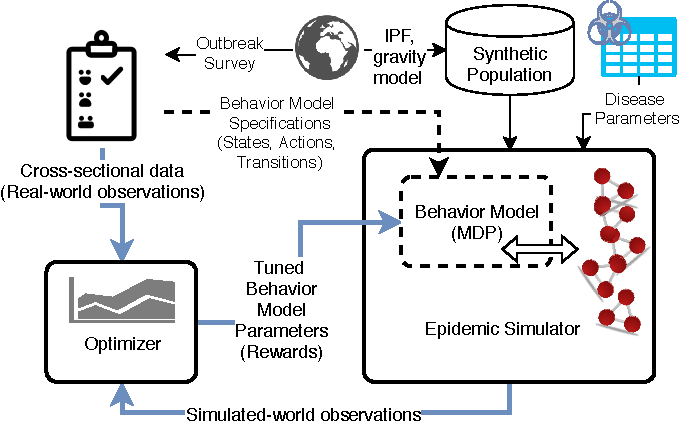
\includegraphics[width=0.8\textwidth]{figures/calibrationproc.pdf}
    \caption{The behavior modeling and calibration approach}
    \label{fig:calib-proc}
    \end{figure}
    
    Figure~\ref{fig:calib-proc} gives a high-level overview of the human behavior modeling and calibration process. There are three inputs to the behavior modeling and calibration approach. First, is the Outbreak Survey, which is a cross-sectional survey of Influenza related behaviors, collected from adults across the United States. The survey was designed to gain insights about people`s experience, beliefs and behaviors with respect to Influenza. In this work, we focus on the behaviors adopted by individuals to avoid getting Influenza. We discuss the survey analysis and the different behaviors in detail in chapter~\ref{ch:survey}. Second, is the Synthetic Population, which is statistically equivalent to a real-world population of a particular geographic region in the United States (e.g., Montgomery county, VA). The Synthetic Population captures the demographics and schedules of its real-world counterpart and is used by the epidemic simulator to simulate the spread of a contagion in the corresponding geographic region. A third input is the disease specific parameters, which are once again used by the epidemic simulator for simulating the corresponding disease within the synthetic population. We also map each behavioral action discovered in the outbreak survey analysis to its implementation in the epidemic simulation. Deciding to adopt an action by an agent may lead to a reduction in the likelihood of the behaving agent getting infected in the epidemic simulation. We discuss the simulation, the synthetic population, disease dynamics models and actions in detail in chapter~\ref{ch:epi-simulations}. 
    
    The behaviors discovered in the outbreak survey analysis along with some of the disease specific details (e.g., health states in the SEIR Influenza progression model) are used to construct the specifications (i.e., the states, actions and transitions) of the agent behavior model (MDP). Within the epidemic simulator, an agent's decision to adopt a set of behaviors is driven by the MDP and the MDP component that drives agent decision making is called the reward function. In this work, we posit that the optimal reward function for the MDP would lead to a close match between the patterns of behavior observed in the simulated and real worlds. To this end, we iteratively tune the parameters of the MDP model used in the epidemic simulator in an optimization loop. We call this the process of behavior model calibration and different optimization algorithms (i.e., Optimizers) lead to different calibration results. We describe the agent-decision making model, the calibration approach and our experiments with three type of optimization approaches in detail in chapter~\ref{ch:decision-model}. Subsequently, we report the main results of this study in chapter~\ref{ch:results} and end with conclusions and future work in chapter~\ref{ch:conclusions}.
    
    The unique contribution of this work is bringing together survey data on behavior, a large-scale simulation that is capable of implementing those same behaviors and an agent decision-making model. The combination of the three aspects leads to a more direct calibration method for the behavior models in our work. The survey provides the relative proportions of a sample of the various behaviors in the population. The simulation in-sync with the agent decision-making model allows us to determine the probability of agents acting in a particular way due to the infectious disease and information flow dynamics in the population. In combination, we can search the space of rewards associated with the behaviors in the MDP using optimization. This optimization can essentially be thought of as an inverse reinforcement learning problem~\cite{ng00irl} where the optimal rewards would lead to a complete match between the population-level phenomenon. The phenomenon of interest being the distribution of behaviors in the outbreak survey human population and the simulated agent population. Next, we discuss past work in the area of behavior modeling from an agent's perspective and from a public health perspective.

	\chapter{Review of Literature} \label{ch:lit_review}
	Efforts at modeling human behavior and decision-making have a long history in the public health and psychology literature. These approaches generally focus on the within-agent decision-making process, such as the Health Belief Model (HBM)~\cite{rosenstock66hbm}, the Theory of Planned Behavior~\cite{ajzen91tpb}, and the Theory of Reasoned Action~\cite{ajzen80understanding}. Health Belief Model suggests that an individual`s decision about preventive action against a disease, depends upon their perceived susceptibility to the disease, perceived severity of the disease and the perceived barriers and benefits (or costs and rewards) associated with taking the preventive action. HBMs have been used and evaluated in countless studies, ranging from decisions on influenza vaccine~\cite{nexoe1999decision,coe2012use,chen2011using} to cancer screening behaviors~\cite{austin2002breast} and preventive actions against smoking~\cite{sharifirad2007effect}. There have also been multiple reviews and meta-analysis of research that uses HBMs~\cite{janz1984health, harrison1992meta, mikhail1981health, daddario2007review}.
	
	Theory of reasoned action assumes that intentions about behaviors are a function of beliefs about the perceived outcome of the behavior. These, beliefs are of two types, behavioral and normative. Behavioral beliefs are the perceived outcomes of behaviors and these reflect an individual`s attitude towards a behavior. Normative beliefs are beliefs about the normative expectations of others and these reflect the individual`s subjective norm about performing a behavior. Theory of reasoned action has been applied to study a diverse range of subjects, ranging from consumer research~\cite{shimp1984theory} to studying and intervening AIDS-related behaviors~\cite{fishbein1989using}.	Theory of planned behavior extends the theory of reasoned action and suggests that human behavior is guided by three aspects, behavioral beliefs, normative beliefs and control beliefs or beliefs about the presence of facilitating or impeding factors which can affect the performance of the behavior. Similar to HBMs, theory of planned behavior has been used in many studies, ranging from smoking cessation behaviors~\cite{norman1999theory} to HPV vaccination uptake~\cite{gerend2012predicting}. There have also been multiple studies which review and evaluate research that applies theory of planned behavior to various domains~\cite{godin1996theory, conner1998extending}. These approaches have been implemented in computational models and have been used to study, changes in human behavior during epidemics like SARS~\cite{durham2011incorporating} and H1N1 influenza~\cite{Durham2012H1N1}, residential water usage~\cite{linkola2013agent}, sexual behavior in adolescents~\cite{orr13health}, vaccination and social distancing decisions~\cite{karimi2015effect} and spatio-temporal adoption of solar photovoltaics~\cite{robinson2013gis}.
	
	The main limitations of these approaches are that the models seem hard to calibrate against data obtained from the real world, since some of the parameters appear to be confounded (e.g., perceived risk and perceived severity). Furthermore, the data required to infer the parameters of these models are hard to obtain. On the other hand, there are many examples of behavior modeling in computational epidemiology and other domains where behaviors are modeled in a counter-factual or prescriptive way. For example, in a study trying to evaluate whether it is better for people to evacuate or shelter in place after a nuclear detonation~\cite{wein10nuclear,parikh16jaamas}, the authors only have to model the counter-factual scenarios where everyone shelters or everyone evacuates.
	
	Similarly, in large-scale simulation studies of flu interventions, modelers generally restrict themselves to assuming that all individuals in the model do the behavior (with some compliance rate). For example, Halloran et al.~\cite{halloran08modeling} studied multiple intervention scenarios in a flu pandemic in the city of Chicago. This work ranked interventions by effectiveness, but did not consider people's typical behavior during flu epidemics.
    
    In a different context, Singh et al.~\cite{singh16bdi} have used the Belief Desire Intention (BDI) framework to create agents which are embedded into large-scale social simulations. Their approach is more focused on the engineering aspects of the problem, such as the agent architecture, modularity, and the design of the simulation platform, than on calibration of the behaviors. They also focus on explainability of agent decision-making and acceptability to the end-users. 
    
    Another relevant stream of research is that of cognitive architectures like Soar~\cite{laird1987soar}, Adaptive control of thought-rational (ACT-R)~\cite{anderson2004integrated}, Connectionist Learning with Adaptive Rule Induction On-line (CLARION)~\cite{sun2006clarion} and Executive Process-Interactive Control (EPIC)~\cite{kieras1997overview} have been aimed at developing human-level intelligence across tasks and domains. These architectures provide specifications about different aspects of human cognition, viz., hierarchical memory systems capable of storing beliefs, goals and experiences, knowledge representations, learning mechanisms and processes that cause behavior. They typically operate in perception-action cycles, where the cognitive agent observes or perceives the environment, searches through its knowledge bank, performs declarative and procedural learning and decides on an action, which is applied to the environment. A recent paper by Kotseruba et al.~\cite{kotseruba2016review} reviews 40 years of research in cognitive architectures and provides a comprehensive summary on the subject. Cognitive architectures are commonly used to create functional agents situated in particular environments and understanding the plausibility of the cognitive architectures themselves~\cite{laird2000creating,laird1998integrating,fleetwood2002modeling,rubinoff1994real,borst2015using,byrne2001act}. These approaches typically model a single agent and due to the focus on complex and general agent behavior are computationally prohibitive when applied to large social simulations.

    A similar approach, typically used to model goal-oriented agents situated in noisy environments is that of reinforcement learning (RL). A RL agent also operates in perception-action cycles, although its decision-making is primarily driven by a reward function. In the RL paradigm, an agent observes the current state of the environment, takes an action, which leads to a new state of the environment and a reward for the agent. Therefore, every state has an associated reward, which is determined by the reward function and the observation-action cycle proceeds in discrete time steps. The agent decision making in this context is modeled as a Markov Decision Process~(MDP)~\cite{white1989markov}. The MDP formalism has existed since the 1950`s and has been extended in many ways. For example, the semi-Markov Decision Process~(SMDP)~\cite{baykal2010semi} formalism models temporally extended actions and is typically used to model agents in stochastic control environments. Another generalization of the MDP formalism is that of partially observable Markov decision process (POMDP)~\cite{kaelbling1998planning}. In an environment defined by a POMDP, an agent cannot observe the state of the environment with complete reliability. In this case, the agent must maintain a memory of previous observations and actions and use it for decision-making. A recent paper by Pynadath et al.~\cite{pynadath16behavior} uses survey data to parametrize a POMDP model of stay/leave decision-making in a disaster response scenario. The study shows how to create the states, actions, environment, and rewards for an agent and then train the agent. The work by Pynadath et al.~\cite{pynadath16behavior} was one of the prime inspirations for this thesis.
    
    In this work, we take a phenomenological approach to modeling preventive behaviors against influenza for a large agent population situated in a social simulation. This leads to development of a MDP based agent-decision making model, which is calibrated against survey-data about influenza avoidance behaviors observed in the real world. We discuss this survey in the next chapter.
    
	\chapter{Outbreak Survey} \label{ch:survey}
	We used data from an epidemiological survey in 2016, aimed at understanding people's experience with the Influenza illness. The survey was administered online by the Gfk~Group~\cite{wiki:wikigfk} to 2165 participants which constituted a nationally representative sample of the United States population, selected from the KnowledgePanel\textregistered. The participants only included adults (people 18 years of age and above) and only included households with at-least one adult occupant. The survey captured demographic information of the participants including age, household income, employment status, education, ethnicity, gender, household and geographic information.
	\begin{figure}
    \centering
    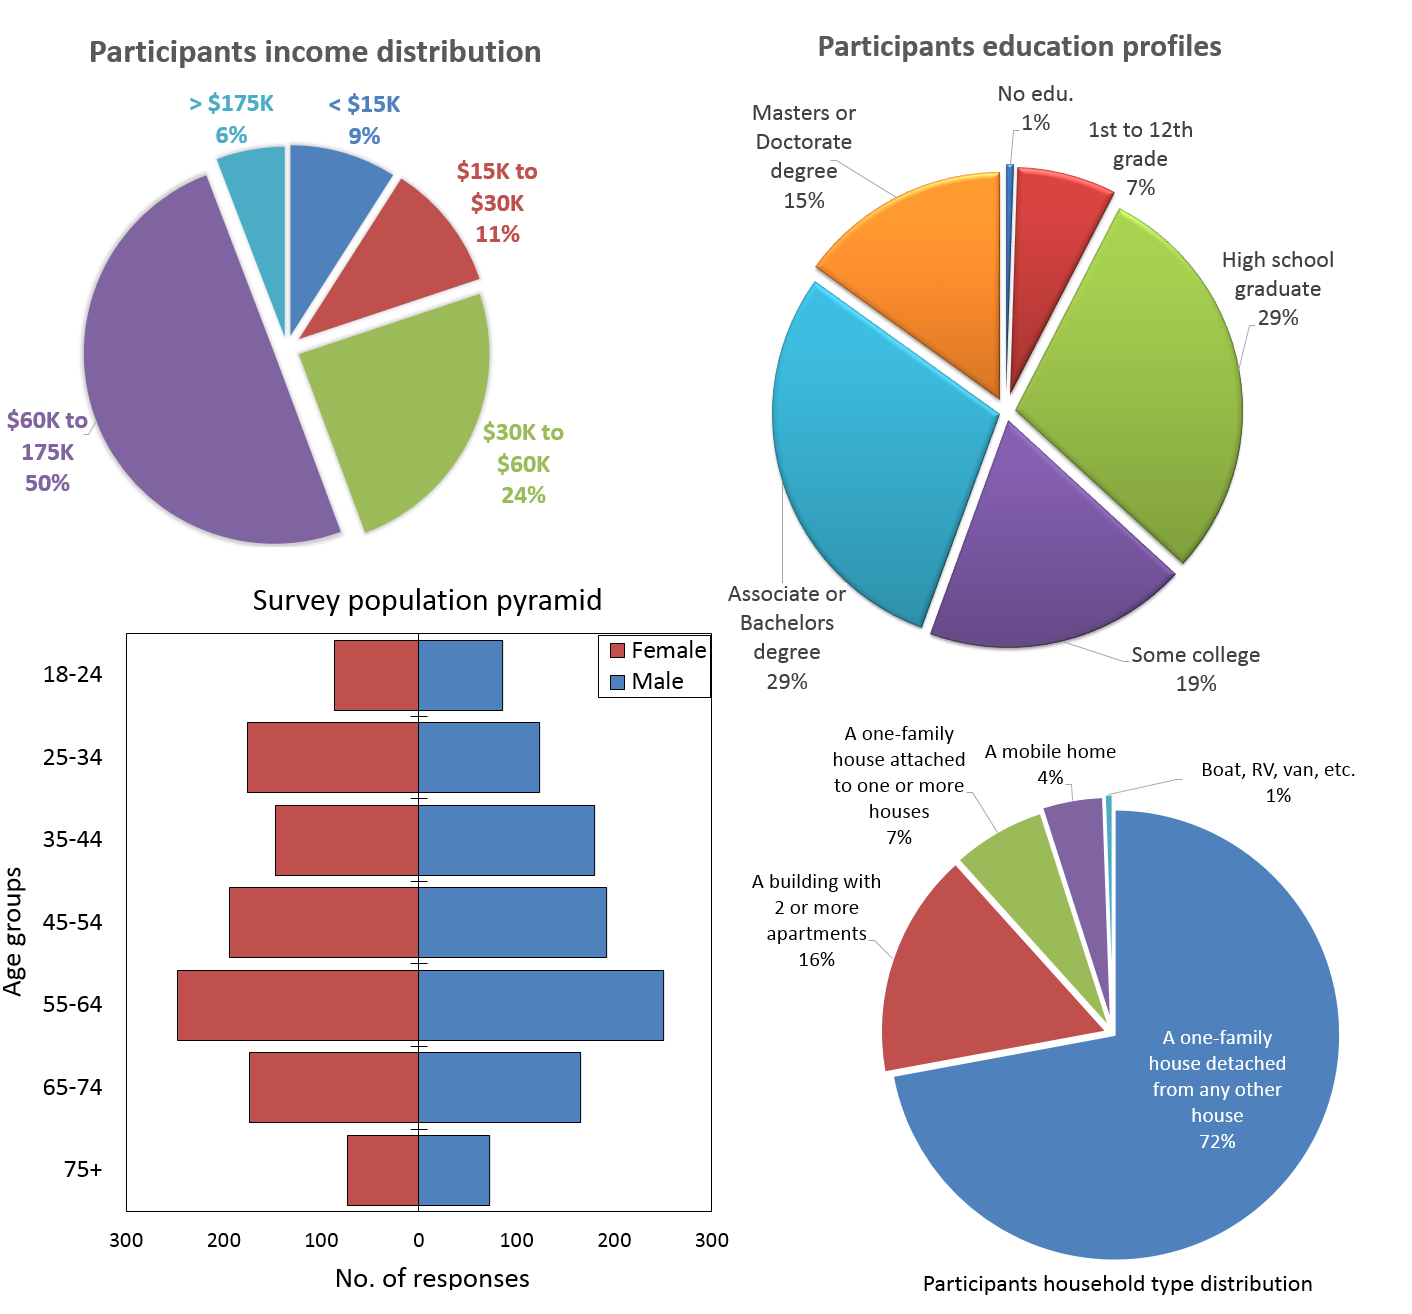
\includegraphics[width=\textwidth]{figures/demographics.png}
    \caption{Demographic distributions of the survey sample}
    \label{fig:demog}
    \end{figure}
	Figure~\ref{fig:demog} shows the distributions of some of these demographics of the surveyed population. The survey also captured participant responses about their health behaviors, risk perceptions, vaccine uptake, and information sources for outbreak updates about Influenza. Of particular relevance to this work were the actions taken by survey participants to avoid getting influenza. These actions are listed below: 
	\begin{enumerate}
	    \item Avoid touching eyes (ATE).
	    \item Avoid touching nose (ATN).
	    \item Avoid touching mouth (ATM).
        \item Wash hands with soap (WHS).
        \item Use hand sanitizers (UHS).
        \item Clean surfaces at home (CSH).
        \item Clean surfaces at work (CSW).
        \item Eat nutritious food (ENF).
        \item Get adequate rest (GAR).
        \item Get recommended vaccine (GRV).
        \item Take preventive medicine e.g. antiviral (TPM).
        \item Use surgical mask to cover nose and mouth (USM).
        \item Avoid contact with people who are sick (ACS).
        \item Avoid crowded places (ACP)
	\end{enumerate}
	\begin{figure}
    \centering
    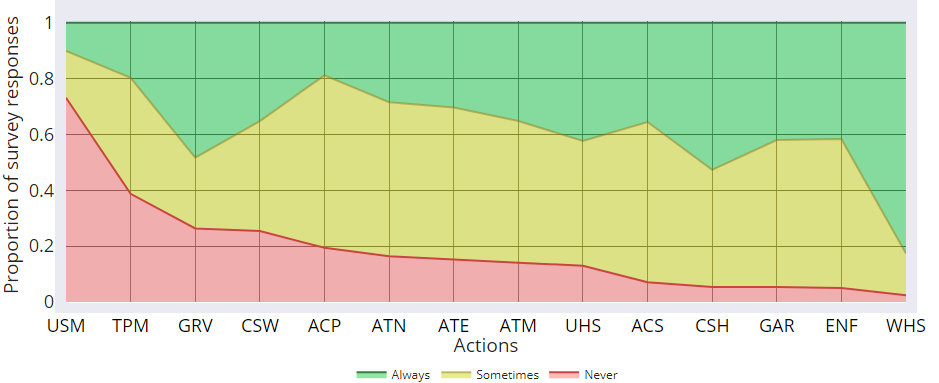
\includegraphics[width=\textwidth]{figures/avoidancebehaviors.png}
    \caption{Distribution of individual avoidance actions in the survey responses}
    \label{fig:avoidance}
    \end{figure}
	For each of these actions, a survey participant chose one of three possible responses: \emph{Never}, \emph{Sometimes}, or \emph{Always}. Figure~\ref{fig:avoidance} gives the distribution of survey responses for the 14 actions. We observe that washing hands with soap is the most popular action, for which more than $82\%$ of the survey participants selected the always response. On the other hand, using surgical mask as an action against Influenza was the least popular action for which only $10\%$ of the participants selected the \emph{always} response. We assume that if a participant selected \emph{Sometimes} or \emph{Always} for an action, they undertake that action in their daily lives to avoid getting an influenza infection. Selecting \emph{Never} for an action implies that the participant does not undertake that action. This simplifying assumption transforms an individual's choice of actions into a binary decision problem. Therefore, an individual either chooses $(1)$ or not chooses $(0)$ an avoidance action.  
    \begin{figure}[H]
    \centering
    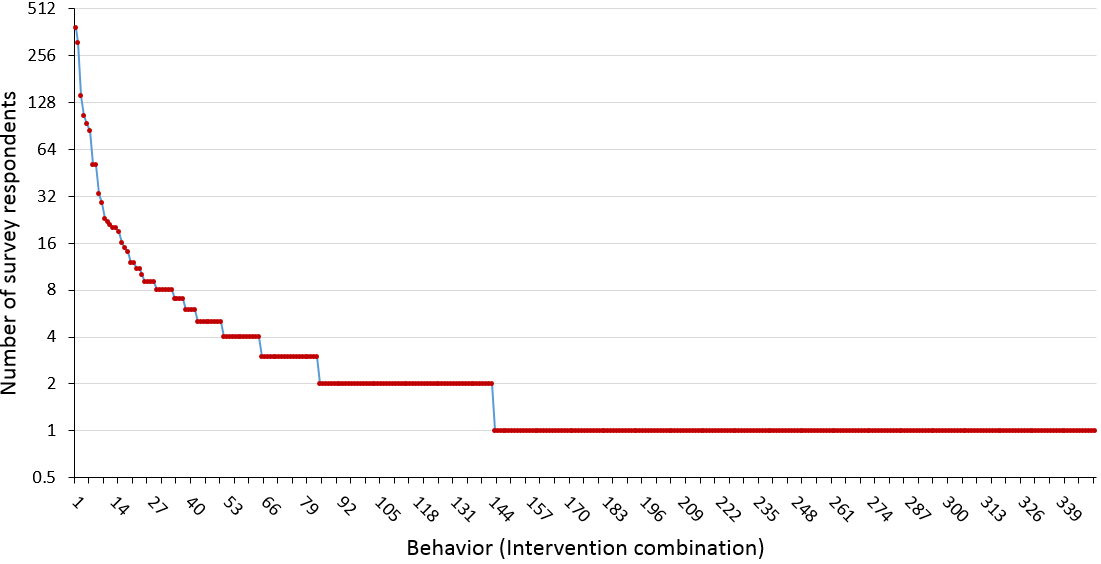
\includegraphics[width=0.8\textwidth]{figures/uniquevectors.png}
    \caption{Distribution of influenza avoidance behaviors observed in the survey.}
    \label{fig:avoidancedist}
    \end{figure}
	Furthermore, an individual can undertake a combination of these actions, for example, one might undertake three actions: avoid touching eyes (ATE), wash hands with soap (WHS) and get recommended vaccine (GRV), so as to avoid getting an influenza infection. We found that there were $351$ such action combinations in the survey responses. From here on, we refer to these avoidance actions as ``actions'' and a combination of avoidance actions as a ``behavior''. Therefore, an individual`s choice of actions constitutes their behavior. Figure~\ref{fig:avoidancedist} gives the frequencies of each of the behaviors observed in the survey, with the data on the vertical axis plotted on $\log_{10}$ scale. Here, the most likely behavior (marked by $1$ on the horizontal axis) corresponds to choosing all actions and is adopted by $385$ survey respondents. The first $10$ behaviors are selected by $60\%$ of the individuals. Additionally, $58\%$ of the behaviors (i.e., behaviors labeled $145$ to $351$ on the horizontal axis) have a frequency of $1$.
    
	
	\chapter{Epidemic Simulations} \label{ch:epi-simulations}
	Large-scale agent-based epidemic simulators work on social contact networks \cite{Glass2008}, to simulate the spread of social contagions such as epidemics, social memes, news and information through these networks. Each node in a social contact network represents a person and each edge represents a temporal contact (i.e., an interaction) between two nodes. The social contact network is thus a dynamic graph where edges or connections between nodes would change based on the schedule followed by individuals that are represented by the nodes. 
	\begin{figure}
    \centering
    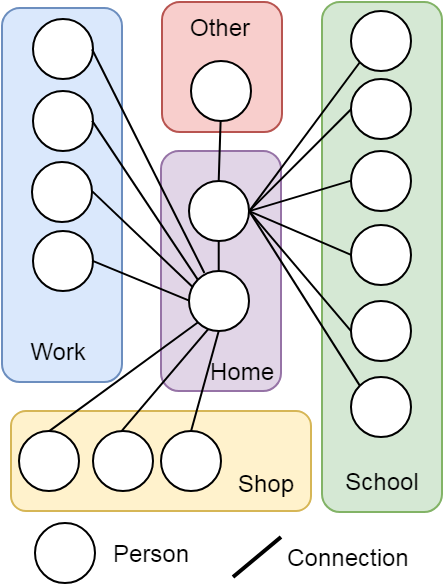
\includegraphics[width=0.4\textwidth]{figures/scn.png}
    \caption{Toy social contact network.}
    \label{fig:scn}
    \end{figure}
	Figure~\ref{fig:scn} shows a toy social contact network with $15$ nodes representing $15$ people and $15$ possible connections (dynamic edges). The blocks represent different locations and the connections may form as the two individuals represented by the nodes in the ``home'' location go about visiting the other $4$ locations in the course of their typical day.
	
	We use Episimdemics \cite{barrett2008episimdemics}, which simulates the spread of infectious diseases through the social contact network corresponding to a synthetic population. Synthetic populations are commonly used in large-scale simulations in multiple domains, including influenza epidemics~\cite{EG+04,parikh14cover}, disaster response~\cite{parikh13nps1}, and more. Next, we describe the synthetic population for Montgomery County in Virginia. We use this synthetic population for all the experiments presented in this work.  
    
    \section{Synthetic population}
    The synthetic population of Montgomery County, VA, is available online~\cite{synthPop2009Montva}. It represents all the residents of Montgomery County and has $77,820$ people grouped into $32,827$ households. Each synthetic individual is assigned a daily activity schedule, with multiple activities in the day. The total number of activities is $429,590$, and these activities are carried out in $26,941$ distinct geographic locations. A location can have different sizes and can contain ``sublocations'' (e.g., rooms within buildings), which can accommodate $25$ to $50$ people. The synthetic population is constructed in a series of steps by integrating data from multiple sources like the American Community Survey (ACS)~\cite{mather2005american}, the National Household Travel Survey (NHTS)~\cite{NHTS11} and HERE (formerly NAVTEQ, for road network data). The process employs algorithms like the iterative proportional fitting (IPF) algorithm~\cite{BBM96} and gravity model~\cite{erlander90gravityModel} to generate a synthetic population which is statistically indistinguishable from the real population. A person-person social contact network can be derived from this synthetic population by assuming that people who are at the same location for an overlapping period of time are in contact with each other. Details of the process can be found in the report by Adiga et al.~\cite{adiga15US}. The resulting social contact network has $77,820$ nodes representing people and over $2$ million edges representing the contacts between these people in Montgomery County, VA. Episimdemics operates on this person-person social contact network, and simulates agents or synthetic individuals as nodes of the network ~\cite{swarup14challenge}. The spread of contagions through the social contact network is modeled through coupled contagion propagation and contagion progression models. We describe these models in the next section.
    
    \section{Contagion propagation and progression models}
    \label{sec:4.2}
    The contagion propagation (inter-host) and contagion progression (intra-host) models used in this work were developed by the National Institutes of Health, Models of Infectious Disease Agent Study (MIDAS) project~\cite{nih09midas}. The inter-host model specifies how an uninfected agent gets exposed to the disease by an infected agent. Such exposures are probabilistic in nature and result from interaction between agents~\cite{barrett2006modeling}. We can use a probability function to model the probability of a susceptible agent $i$ getting infected based on its immediate social contact network neighbors, disease parameters, agent-specific parameters and environment-specific parameters. The probability function is defined as,
    \begin{align}
    p_i = 1 - \exp \Bigg(  \tau \sum_{r \in R} N_r \ln (1-r s_i \rho) \Bigg).
    \label{eqn:1}
    \end{align}
    Here, $p_i$ is the probability of a susceptible agent $i$ getting infected, $\tau$ is the duration of exposure in minutes, which is the time spent by agent $i$ at the same location as $N_r$ (collocated) infectious agents, $R$ is the set of infectivities ($r$s) of each of the $N_r$ infectious agents collocated with the susceptible agent $i$, $s_i$ is the susceptibility of $i$ and $\rho$ is the disease transmission rate, which is the probability of a single completely susceptible agent getting infected by a single completely infectious agent through one minute of contact \cite{barrett2007modeling}. This model ensures that the presence of multiple infected agents in the neighborhood of a susceptible agent increases the agent`s probability of getting infected. Conversely, absence of infected neighbors makes the probability of getting infected for a susceptible agent equal to zero. 
    \begin{figure}
    \centering
    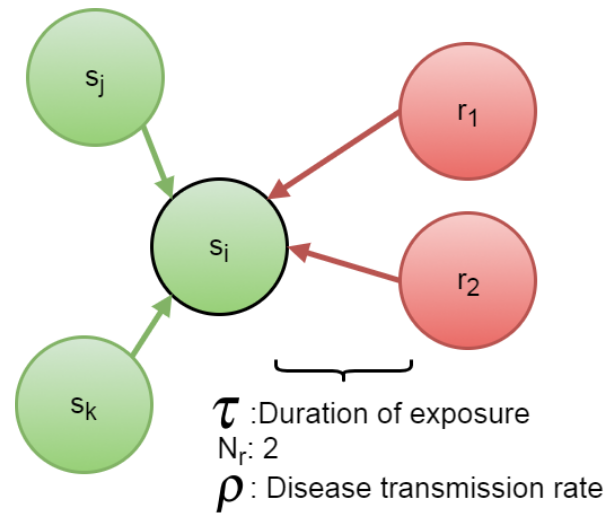
\includegraphics[width=0.4\textwidth]{figures/dpm.png}
    \caption{Contagion propagation model.}
    \label{fig:dpm}
    \end{figure}
    
    Figure~\ref{fig:dpm} shows a graphical representation of the inter-host disease propagation model. Here, the green nodes represent susceptible individuals and red nodes represent infectious individuals. Each susceptible node has an associated susceptibility parameter, which is depicted at the center of the green colored nodes. Similarly, each infectious node has an associated infectivity parameter, depicted at the center of the red colored nodes. Now, using the disease propagation model defined in equation~\ref{eqn:1}, we can compute the probabilities of infection for each of the susceptible nodes in figure~\ref{fig:dpm}. Since, nodes $j$ and $k$ do not have any infectious neighbors their probability of infection comes out to be $p_j = p_k = 1 - \exp (\tau * 0 ) = 1 - 1 = 0.0$. On the other hand, since the node $i$ has two infectious neighbors, its probability of infection comes out to be non-zero, i.e., $p_i = 1 - \exp (\tau * (\ln (1 - (r_1 s_i \rho)) + \ln (1 - (r_2 s_i \rho))))$. Table~\ref{table:1} shows the specific values of the Influenza propagation model parameters used in this work. 
    \begin{table}[!t]
    \renewcommand{\arraystretch}{1.3}
    \centering
    \caption{Variable values used in the influenza propagation model}
    \begin{tabular}{|l|c|}
    \hline
    \multicolumn{1}{|c|}{\textbf{Variable}} & \textbf{Value}  \\ \hline
    $r$ in Susceptible states & $0.0$ \\ \hline
    $r$ in Exposed state & $0.0$ \\ \hline
    $r$ in Infectious state & $1.0$ \\ \hline
    $r$ in Recovered state & $0.0$ \\ \hline
    $s_i$ in Susceptible states & $[0.574649378, 1.0]$ \\ \hline
    $s_i$ in Exposed state & $0.0$ \\ \hline 
    $s_i$ in Infectious state & $0.0$ \\ \hline
    $s_i$ in Recovered state & $0.0$ \\ \hline
    $\rho$ & $1.0$ \\ \hline
    \end{tabular}
    \label{table:1}
    \end{table}
    
    Upon being infected, the progression of the disease within an agent is modeled using the disease progression or intra-host model. This model is a Probabilistic Timed Transition System (PTTS), which is a finite state machine with probabilistic and timed state transitions~\cite{bisset2009modeling}. The specific PTTS we use in this work is based upon the well-known SEIR compartmental model, typically used for mathematical modeling of infectious diseases. Figure~\ref{fig:disease} shows a schematic of the disease PTTS that we have used in this work for simulating the progression of Influenza within an individual. 
    \begin{figure}
    \centering
    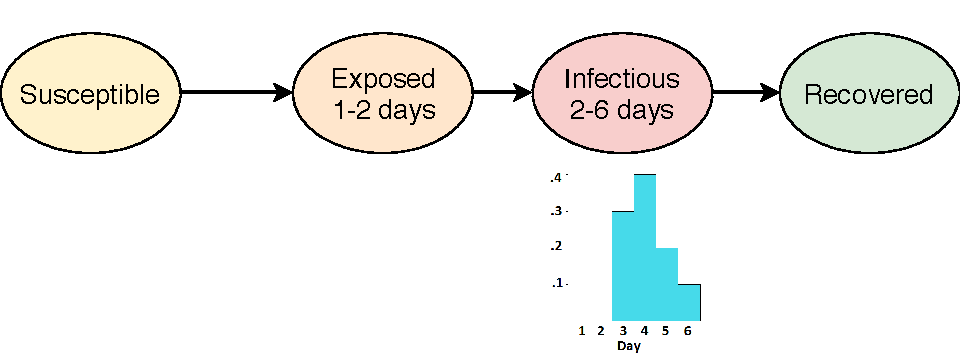
\includegraphics[width=0.8\textwidth]{figures/disease-fsm.pdf}
    \caption{Within-host disease PTTS}
    \label{fig:disease}
    \end{figure}
    
    Each agent remains in the susceptible (S) state until it encounters one or more infected agents in its social contact network neighborhood. Then we calculate $p_i$ based on the susceptibility of agent $i$ (which in turn depends on its behaviors) and the number of infected agents in the neighborhood ($N_r$). Agent $i$ is then set to be exposed with probability $p_i$. In this case, the probability of getting infected (i.e., $p_i$) increases for the susceptible agent. The value of $p_i$ is used to determine whether or not the disease was transmitted to the susceptible agent using a random draw from the uniform distribution $\mathcal{U}(0,1)$. If the random draw comes out to be less than the value of $p_i$ for an agent, it is considered as a successful transmission. 
    
    In this case, the agent`s disease PTTS transitions to the exposed (E) state from the Susceptible (S) state. An agent remains in the exposed (E) state for a period of one to two days after which it transitions into the infected (I) state. The exact duration (in hours) for which an agent remains in the exposed state before transitioning to infected state is once again determined by a random draw from the uniform distribution $\mathcal{U}(24,48)$. However, a transition to the infected state is guaranteed to happen in $48$ hours of being infected. Once an agent transitions to the infected state, it remains infectious for a period of two to six days, after which it transitions to the recovered (R) state. The duration (in days) for which an agent stays in the infected state is determined using the distribution: ($3$ days$/4$ days$/5$ days$/6$ days), ($0.3/0.4/0.2/0.1$) as shown in the histogram presented in Figure~\ref{fig:disease}. Agents in the infectious state can spread the infection to other susceptible agents, which come in contact with them through the social contact network as evident by the infectious agent's infectivity of $(1.0)$. An agent in the recovered state is no longer contagious and cannot get new infections.
    
    \section{Information Contagion}
    The intra-host and inter-host models can also be used to simulate the propagation of other contagions in the social contact network. People's decisions about preventive behaviors can be dependent upon network phenomenon, like changing their preventive behaviors upon receiving news about an outbreak. We model a simple contagion, called the information contagion, which carries news about the outbreak in the agent population. This is used to trigger decision making about the disease avoidance behaviors in the agents. Figure~\ref{fig:information} shows the PTTS which models the information contagion about the influenza outbreak. 
    \begin{figure}
    \centering
    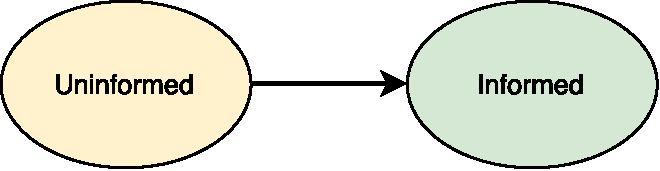
\includegraphics[width=0.45\textwidth]{figures/information-fsm.pdf}
    \caption{Within-host information PTTS}
    \label{fig:information}
    \end{figure}
    This within-host information PTTS functions similarly to the disease PTTS, but has only two states (i.e., uninformed and informed). Initially, all agents are in the ``uninformed'' state, but once an agent gets infected by the influenza contagion, its information state changes to ``informed''. Agents in the contact network neighborhood of an infected agent get informed about the outbreak faster than they get infected. This is achieved by having an information contagion susceptibility two times the susceptibility to the disease contagion. This results in the information about the disease outbreak spreading faster than the disease itself. The information contagion model reflects the role of peer influence in an individual's decision-making. Table \ref{table:2} lists the specific values of the variables that were used for the information contagion in our simulations.
    \begin{table}[!t]
    \renewcommand{\arraystretch}{1.2}
    \caption{Variable values used in the info. propagation model}
    \centering
    \begin{tabular}{|l|c|}
    \hline
    \multicolumn{1}{|c|}{\textbf{Variable}} & \textbf{Value}  \\ \hline
    $r$ in Uninformed state & $0.0$ \\ \hline
    $r$ in Informed state & $1.0$ \\ \hline
    $s_i$ in Uninformed state & $2.0$ \\ \hline
    $s_i$ in Informed state & $0.0$ \\ \hline 
    $\rho$ & $1.0$ \\ \hline
    \end{tabular}
    \label{table:2}
    \end{table}
    Upon receiving information about the outbreak, an agent can decide to undertake one or more actions to avoid getting the disease. In the context of influenza, an agent can undertake any of the $351$ combinations of the $14$ actions that were discussed in Section 3. 
    
    \section{Actions}
    
    Until now, we have looked at processes that are sufficient to simulate the spread of contagions like diseases and diffusion of information in large synthetic populations. Here, we describe how individual avoidance actions and their combinations are implemented in the simulation. We assume that adopting an action can affect an individual in multiple ways. 
    
    First, adopting hygienic practices like, washing hands with soap and using hand sanitizers in the real world, reduce an individual`s susceptibility to the disease. Therefore, when an agent decides to adopt a hygienic practice in an epidemic simulation, we simply reduce its susceptibility parameter. Additionally, adopting more actions would make an individual much more protected in the real world. This implies that the reduction in susceptibilities always adds up, i.e., for an agent, adopting more actions results in larger reduction in its susceptibility. 
    
    Second, certain actions lead to a change in an individual`s schedule, which can affect the structure of the social contact network of the population under consideration. For example, if an individual decides to completely stop visiting any crowded place upon receiving information about a disease outbreak, the likelihood that it will get an infection from any of the said crowded places becomes zero. Such actions are broadly classified as social distancing and they control disease spread by making the nodes in the social contact network less connected. 
    
    Third, vaccines are generally thought of as making individuals immune to the particular disease. Therefore, in an epidemic simulation any agent deciding to adopt vaccination as an avoidance action would become immune to the disease. This translates to transitioning the within-host PTTS for the agent to the ``Recovered'' state. While this is rather straightforward to implement, vaccine efficacy can vary because of a myriad of factors. For example, different strains of the circulating pathogen, host factors like age, prior exposure to the pathogen, time since vaccination and vaccine characteristics like live or inactivated, mode of delivery~\cite{mcneil2012over}. This is more often than not true in the case of Influenza. Hence, for the sake of simplicity we can think of vaccination as just another hygienic practice that reduces the susceptibility to the disease, instead of making the agent immune to the disease.
    
    Finally, an individual can adopt a combination of all or any of these avoidance actions and this combination constitutes its behavior. Therefore, adopting a particular action combination can reduce the susceptibility of an agent to the disease as well as affect its contact neighborhood (which affects the overall social contact network of the synthetic population being simulated). It is important to note that measuring or estimating the exact reduction in susceptibility caused by an action is difficult, but we can rely on domain-experts for this information. In this work, we assume that if an action is easy to take then a lot of people will adopt it, but it will also have a smaller effect on the susceptibility to the disease. Hence, the reduction in susceptibility due to an action is assumed to be an inverse function of the number of survey participants who responded as undertaking that action. 
    
    Therefore, upon receiving information about the Influenza outbreak, a susceptible agent can decide to undertake an action combination, (i.e., a behavior) using the MDP decision-making model. In order to account for the $351$ possible behaviors that can be decided upon, we modify the within-host PTTS shown in figure~\ref{fig:disease} to the one shown in figure~\ref{fig:disease-behavs}.
    
    \begin{figure}
    \centering
    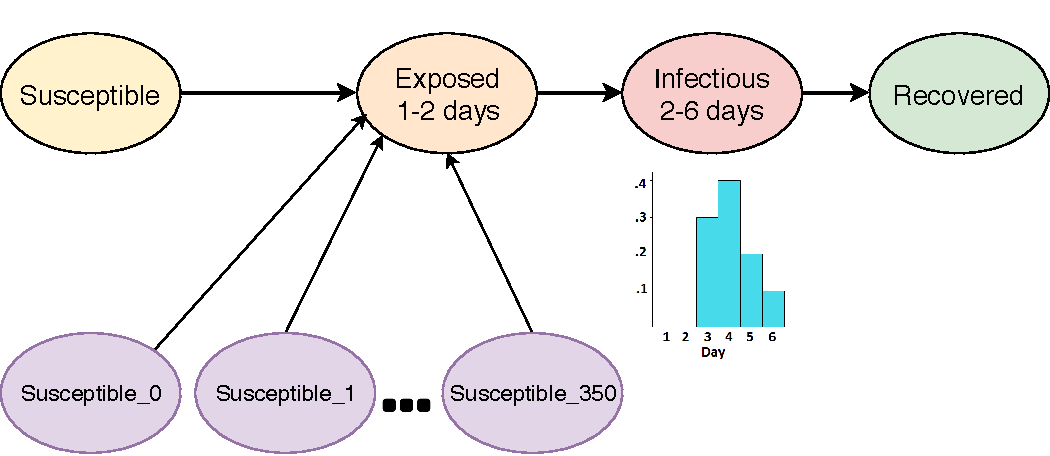
\includegraphics[width=0.8\textwidth]{figures/disease-fsm-behavs.pdf}
    \caption{Modified within-host disease PTTS}
    \label{fig:disease-behavs}
    \end{figure}
    
    Once an agent has decided on a behavior, their disease PTTS is transitioned to one of the susceptible states (shown in purple) in figure~\ref{fig:disease-behavs}. In other words, if an agent decides to adopt behavior $b$ the PTTS corresponding to that agent is transitioned to the Susceptible\_$b$ state. Each of these $351$ susceptible states implies a lower susceptibility towards influenza for the agent than the original Susceptible (S) state. Additionally, if the behavior contains a social distancing action like avoiding crowded places or avoiding contact with people who are sick, the schedule of the behaving agent is changed to reflect the respective action. 
    
    We note that the assumed inverse relationship between ease of undertaking an action and the reduction in susceptibility associated with it may or may not hold in the real world. This assumption and the simplified disease and information models used in this study are not central to the behavior modeling and calibration methodology and merely serve the purpose of demonstrating the approach. Given the availability of quantitative data linking actions with reduction in susceptibility, one can easily forgo this assumption, without affecting the overall behavior modeling and calibration approach. Additionally, the disease and information models can be substituted with more complex variants for modeling any other kind of infectious disease as well as network phenomenon like, peer influence. In the next chapter, we define the agent decision-making model, which is central to the work presented herein.

    \chapter{Agent decision making model}\label{ch:decision-model}
    We define the Markov Decision Process (MDP) driving agent decision making as a $4$-tuple $\big<\mathcal{S,B,P,R}\big>$. The state space $\mathcal{S}$ consists of all the possible health and information states for an agent, which are reflected in the states of the within-host disease and information PTTSs shown in figures~\ref{fig:disease-behavs}~and~\ref{fig:information}. Therefore, if the sets of possible health and information states are $S_H$ and $S_I$ respectively, the total number of possible states for an agent are $|S_H| X |S_I|$. In this work, we have kept $S_H = 355$ (i.e., the four S, E, I and R states and the 351 Susceptible states) and $S_I = 2$, resulting in a total of $710$ possible states for an agent. The behavior space $\mathcal{B}$ consists of the $351$ behaviors that an agent can adopt, which were observed in the outbreak survey. The transition model $\mathcal{P}$ determines the transitions in the state space $\mathcal{S}$, given a behavior $b \in \mathcal{B}$. In other words, $\mathcal{P}_b(s,s') = P(s_{t+1} = s' | s_t = s, b_t = b)$ defines the probability that for an agent adopting behavior $b$ in state $s$ at time $t$ will lead to state $s'$ at time $t+1$. In the case of epidemic simulations, these transition probabilities are dependent on the disease and information diffusion happening in the simulation, which are complex phenomena. Hence, in this work the transition function $\mathcal{P}$ of the MDP is intensively specified by the simulation model and cannot be computed extensively. 
    
    Lastly, the reward function $\mathcal{R}_b(s, s')$ in a MDP determines the reward received by an agent upon transitioning form a state $s$ to state $s'$, due to behavior $b$, here, $s, s' \in \mathcal{S}$ and $b \in \mathcal{B}$. In the context of this work, we associate not being infected i.e., remaining in one of the susceptible states with a positive reward for an individual and adopting an avoidance behavior with a negative reward (or cost). Thus, on a particular day in the simulation, if an agent remains in one of the susceptible states they receive a positive reward of $+1$. Additionally, if the agent has adopted any of the avoidance behaviors we subtract the cost associated with that behavior from the net reward collected by the agent. The key idea here is that, an agent can select a behavior, which will reduce its immediate reward, but will also lead to a lower susceptibility to the disease. This would increase its odds of remaining in one of the susceptible states, thereby increasing its likelihood of collecting future rewards. Since, in our case the immediate reward is only dependent on the current state and the selected behavior, we can state the immediate reward associated with behaviors $b$ and state $s$ as $\mathcal{R}_b(s)$.

    The behavioral decision for a susceptible and informed agent is to select an optimal behavior such that its accumulated reward over the remaining simulation duration is maximized. On a particular day in the simulation, this behavioral decision depends on the agent`s probability of getting exposed and the cost associated with the $351$ behaviors. Taking these aspects into account, we define a value function $V_d(b)$ associated with a behavior $b$ on a day $d \in [1,D]$ as follows,
    \begin{align*}
    V_d(b) &= \sum_{i=d}^D \bigg\{ \mathbb{E} [\mathcal{R}_b(s_i)] \bigg\}  \\
        &= \sum_{i=d}^D \bigg\{ (1 - cost_b) * P(s_i \in \mathcal{S}_{Susceptible}) \bigg\} 
    \end{align*}
    Here, $D$ is the total number of days for which the epidemic is being simulated, $\mathcal{R}_b(s_i)$ is the immediate reward associated with the state $s_i \in \mathcal{S}$ and behavior $b \in \mathcal{B}$. Therefore, the value function associated with behavior $b$ on day $d$ is the sum of all expected rewards from the current day $d$ until the end of the epidemic simulation. Assuming $\mathcal{S}_{Susceptible} \subset \mathcal{S}$ is the set of all states in the MDP, in which the agent`s health state corresponds to one of the susceptible states defined in the disease PTTS. The expected daily reward collected by an agent, who has adopted behavior $b$ and is in the state $s \in \mathcal{S}_{Susceptible}$ of the MDP, can be given by the $+1$ reward for being susceptible (i.e., not being exposed to the disease) minus $cost_b$, which is the cost associated with the behavior $b$. Since, this reward is only valid if the state $s \in \mathcal{S}_{Susceptible}$, we also need factor in the probability that the agent`s state $s_i$ on day $i$ belongs to the $\mathcal{S}_{Susceptible}$ set. We do this by multiplying the expected reward with the $P(s_i \in \mathcal{S}_{Susceptible})$. In addition, as the reward for being in a state $s' \notin \mathcal{S}_{Susceptible}$ is zero; we do not consider these rewards in our formulation of the value function. 
    
    As the membership of a state $s$ in the set $\mathcal{S}_{Susceptible}$ is only determined by the disease PTTS, we can further simplify the value function as follows,
    \begin{align}
    V_d(b) &= \sum_{i=d}^D \bigg\{ (1-cost_b) * (1 - P_i(S \rightarrow E|b)) \bigg\} 
    \label{eqn:valfn}
    \end{align}
    Here, $P_i(S \rightarrow E|b)$ is the probability of any agent in the population transitioning from one of the susceptible states ($S$) to the exposed state ($E$) on the $i^{th}$ day of the simulation, given that the agent undertakes the behavior $b$. The probability of not transitioning to the exposed state on day $i$ can hence be written as, $1 - P_i(S \rightarrow E|b)$). Since the goal of every agent is to maximize the collected reward, the optimal behavior choice for every susceptible and informed agent on day $d$ will be the one that maximizes the value function defined in the equation \ref{eqn:valfn}. 
    
    As we have discussed earlier that the transition function $\mathcal{P}$ of the MDP cannot be computed extensively, we can only estimate the probability term $P_i(S \rightarrow E|b)$ for computing the value function. We estimate $P_i(S \rightarrow E|b)$ for an agent on day $i$ of the epidemic simulation, based on the extent to which the disease has spread through the population as shown below,
    \begin{align}
    P_i(S \rightarrow E|b) &= f_i  \prod_{t=0}^{(i-1)} (1 - f_t)
    \label{eqn:2}
    \end{align}
    Here, $f_i$ is the fraction of agents in the population that have transitioned to the exposed state by the day $i$ (exposed agents) given that the entire agent population has adopted the avoidance behavior $b$. Since, $f_i$ is an agents best estimate of the probability of being exposed to the disease on day $i$, we can interpret \ref{eqn:2} as the probability that the agent did not get exposed to the disease before day $i$ (i.e., the agent remained susceptible from from day $0$ till day $i-1$) and got exposed on the $i^{th}$ day. Since an agent does not have access to the full state of the simulated population, we use a simple differential equation model of the SEIR process \cite{hethcote1976qualitative} to estimate the fractions of exposed agents in the population on subsequent epidemic simulation days, for a particular behavior $b$. The following differential equations describe the ODE model,
    \begin{align*} 
    		\frac{dS}{dt} &= \mu - (\beta I + \mu) S, \\
    		\frac{dE}{dt} &= \beta S I - (\mu + \sigma) E, \\
    		\frac{dI}{dt} &= \sigma E - (\mu + \gamma) I, \\
    		\frac{dR}{dt} &= \gamma I - \mu R.
    \end{align*}
    \begin{table}[!t]
    \renewcommand{\arraystretch}{1.2}
    \caption{Variable values used in the ODE model}
    \centering
    \begin{tabular}{|l|c|}
    \hline
    \multicolumn{1}{|c|}{\textbf{Variable}} & \textbf{Value}  \\ \hline
    ODE simulation duration & $100$ days\\ \hline
    $\mu$ & $0.0$ \\ \hline
    $\beta$ & $[0.3,0.6]$ \\ \hline
    $\gamma$ & $0.125$ \\ \hline
    $\sigma$ & $0.5$ \\ \hline
    Initial proportion of exposed agents & $0.0001$ \\ \hline 
    Initial proportion of infectious agents & $0.0001$ \\ \hline
    Initial proportion of susceptible agents & $0.9998$ \\ \hline
    Initial proportion of recovered agents & $0.0$ \\ \hline
    \end{tabular}
    \label{table:ode}
    \end{table}
    Here, $S,E,I$ and $R$ represent the number of susceptible, exposed, infectious and recovered agents in a population. $\mu$ and $\beta$ represent the natural mortality and transmission rates respectively. $\gamma$ and $\sigma$ represent the recovery and infection rate respectively. For the purpose of this study, the values of variables used in the ODE model are listed in Table~\ref{table:ode}. We assume the natural mortality rate to be zero and the values of other variables are taken from a standard ODE based SEIR model~\cite{keeling2008modeling}. Also, similar to the disease PTTS, repeated exposure is not modeled in this work because once an agent gets infected and recovers, they cannot be infected again by the same strain of influenza virus. 
    
    The ODE model generates epidemic curves or ``epicurves'', which represent the fraction of exposed individuals in the population over time. We can use these fractions to estimate $P_i(S \rightarrow E|b)$ as per equation~\ref{eqn:2}. We assume that adopting one of the $351$ behaviors would lead to a change in the transmission rate ($\beta$), while the recovery and infection rates ($\gamma$ and $\sigma$) would remain unchanged. This assumption leads to a range of $\beta$ values in the interval of 0.3 to 0.6. This is the reason why we have specified $\beta$ as a range in table~\ref{table:ode}, instead of a single value. Each of these $\beta$ values corresponds to one of the 351 behaviors and results in a different epicurve. Figure \ref{fig:epicurves} shows 21 of the 351 Epicurves generated by the ODE model for the avoidance behaviors discovered in the outbreak survey.
    \begin{figure}
    \centering
    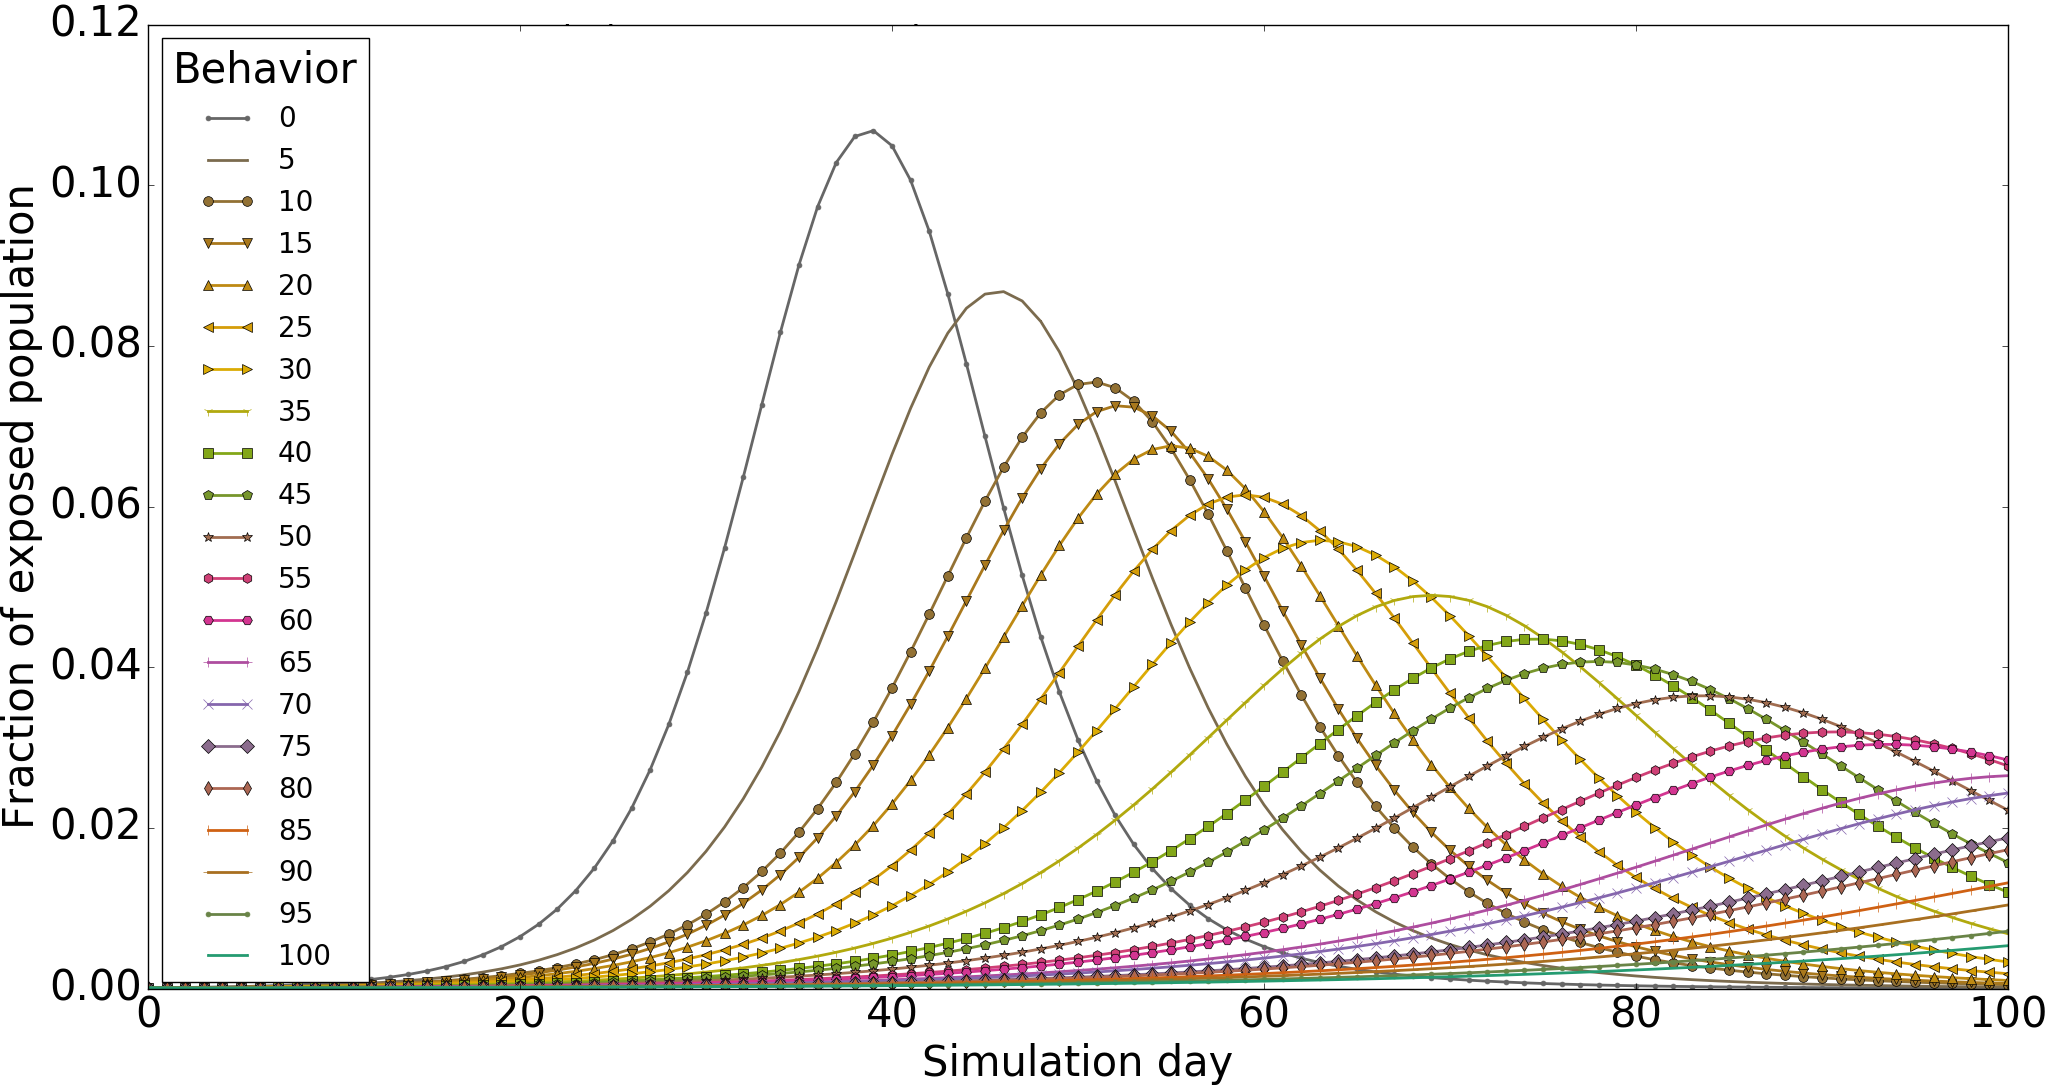
\includegraphics[width=\textwidth]{figures/epicurves.png}
    \caption{Epicurves generated by the ODE model for 21 of the 351 behaviors}
    \label{fig:epicurves}
    \end{figure}
    
    On each day of the simulation, each agent has to choose a behavior based on its estimate of its probability of getting infected. Since, we can now estimate $P_i(S \rightarrow E|b)$, we can use equation~\ref{eqn:valfn} to compute the values associated with the $351$ behaviors and the agent can select the optimal behavior $b$ for any day $d$ in the simulation such that,
    \begin{align}
        max_{b} V_d(b)
    	\label{eqn:optb}
    \end{align}
    In the course of a simulation day any susceptible agent who has received information about the outbreak would choose to undertake the optimal behavior. The MDP, the epicurves generated by the ODE model and the behavior selection process together constitute the agent decision-making model or behavior model.  
    
    Note that, the costs associated with the behaviors are still unknown and need to be determined for the behavior model to operate. The survey described in chapter~\ref{ch:survey} gives information about the behaviors that people do, but does not provide any pointers about the perceived cost of these behaviors. Additionally, it is important to understand that these costs do not refer to the financial or dollar costs that might be associated with a set of actions; rather it`s an implicit behavior model parameter which discounts the immediate rewards generated by the reward function $\mathcal{R}$ of the MDP.
    
    As an example, people may not prefer to use surgical masks, even if they may provide the best protection against infection, because of perceived low social acceptability of wearing face masks. We posit that these costs are a parameter of the behavior model, which can be tuned such that the distribution of behaviors adopted by agents in the epidemic simulation would match the distribution of behaviors observed in the real world. To determine these implicit costs, we calibrate the model by treating it as an inverse reinforcement learning problem where we use the epidemic simulator in a loop with an optimizer to estimate the optimal costs. This is described in the next section.
    
    \section{Behavior model calibration}
    We consider the distribution of behaviors selected by participants of the outbreak survey as our real world observations. We calibrate the $cost_b$ parameters associated with behaviors of the behavior model to minimize the mean squared error (MSE) between the simulation and survey distributions of the $351$ observed behaviors. Thus, the objective of behavior model calibration is to compute an optimal cost, $cost_b^*$, associated with behavior $b$, $\forall b \in \mathcal{B}$. This can be viewed as an inverse reinforcement learning problem~\cite{ng2000algorithms} where given the States, Actions and Transitions (i.e., \big<$\mathcal{S,A,P}$\big>) of an MDP, along with some estimate of an optimal policy $\pi^*$, an optimal reward function $\mathcal{R}$ is estimated. We specify the costs associated with the $351$ behaviors in a vector $C$, such that each element $c_i \in C$ corresponds to $cost_i$ $\forall 0 \le i \le 350$. The objective function $J(C)$ is defined as follows,
    \begin{align}
        J(C) &= \frac{1}{2 * |C|} \sum_{b \in B}\bigg[ N_{C_b} - N_{b} \bigg]^2
    		\label{eqn:objfn}
    \end{align}
    \begin{align}
    		C^* &= \argmin_C J(C) 
    		\label{eqn:optc}
    \end{align}
    Here, $N_{C_b}$ is the proportion of agents which decide to follow the behavior $b$ in the simulation, given the cost vector $C$. $N_{b}$ is the proportion of survey respondents that selected behavior $b$. Note that the objective $J(C)$ is a modified form of the objective function~\ref{obj-func} defined in the \textsc{BehavAssign} problem. The modifications are that the values of $\upalpha$ and $\upbeta$ are set to $1$ and $0$ respectively. The other modification is that instead of using a sum of absolute differences between the behavior proportions observed in the simulation and the survey (i.e., $\sum_{i=1}^{m}|p_i - \hat{p_i}|$) we use mean squared error (i.e., $ \frac{1}{2 * m}\sum_{i=1}^{m} (p_i - \hat{p_i})^2$). 
    
    In equation (\ref{eqn:optc}), $C^*$ is the optimal cost vector, which minimizes the objective function $J(C)$, thereby minimizing the difference between the distribution of behaviors produced by the agent decision model used in the simulation and those observed in the survey data. Note that $N_{C_b}$ is derived from the simulator and it depends on the simulation inputs like, the social contact network, the disease and information characteristics, as well as the behavior model inputs like the cost vector $C$. We can think of the simulator as a function $\mathscr{S}$ which transforms the various simulation and behavioral model inputs to proportions of agents following the different behaviors, i.e., $N_{C_b}$. In other words, the function $\mathscr{S}(\cdot, C)$ represents the simulator output corresponding to $N_{C_b}$ (i.e., $\mathscr{S}(\cdot, C) = N_{C_b}$) and we can re-write equation~\ref{eqn:objfn} as follows,
    \begin{align}
        J(C) &= \frac{1}{2 * |C|} \sum_{b \in B}\bigg[ \mathscr{S}(\cdot, C) - N_{b} \bigg]^2
    	\label{eqn:objfn2}
    \end{align}
    If we had an extensive mathematical definition of the simulator $\mathscr{S}$, and if the definition turned out to be a differentiable function, we can differentiate $J(C)$ with respect to $C$ and use any of the popular gradient based optimization techniques to find the optimal cost vector $C^*$ which minimizes $J(C)$. We can say that the behavior model is calibrated with the survey, once the optimization converges. However, as we have discussed earlier an extensive mathematical definition of $\mathscr{S}$ does not exist, hence we can only use gradient-free optimization methods to estimate the optimal cost vector $C^*$. We experiment with three such gradient-free optimization methods, viz. Numerical Gradient Descent (NGD), Cross Entropy (CE) method and Smoothed-Cross Entropy (SCE) method, which we describe next. 
    \begin{figure}[H]
    \centering
    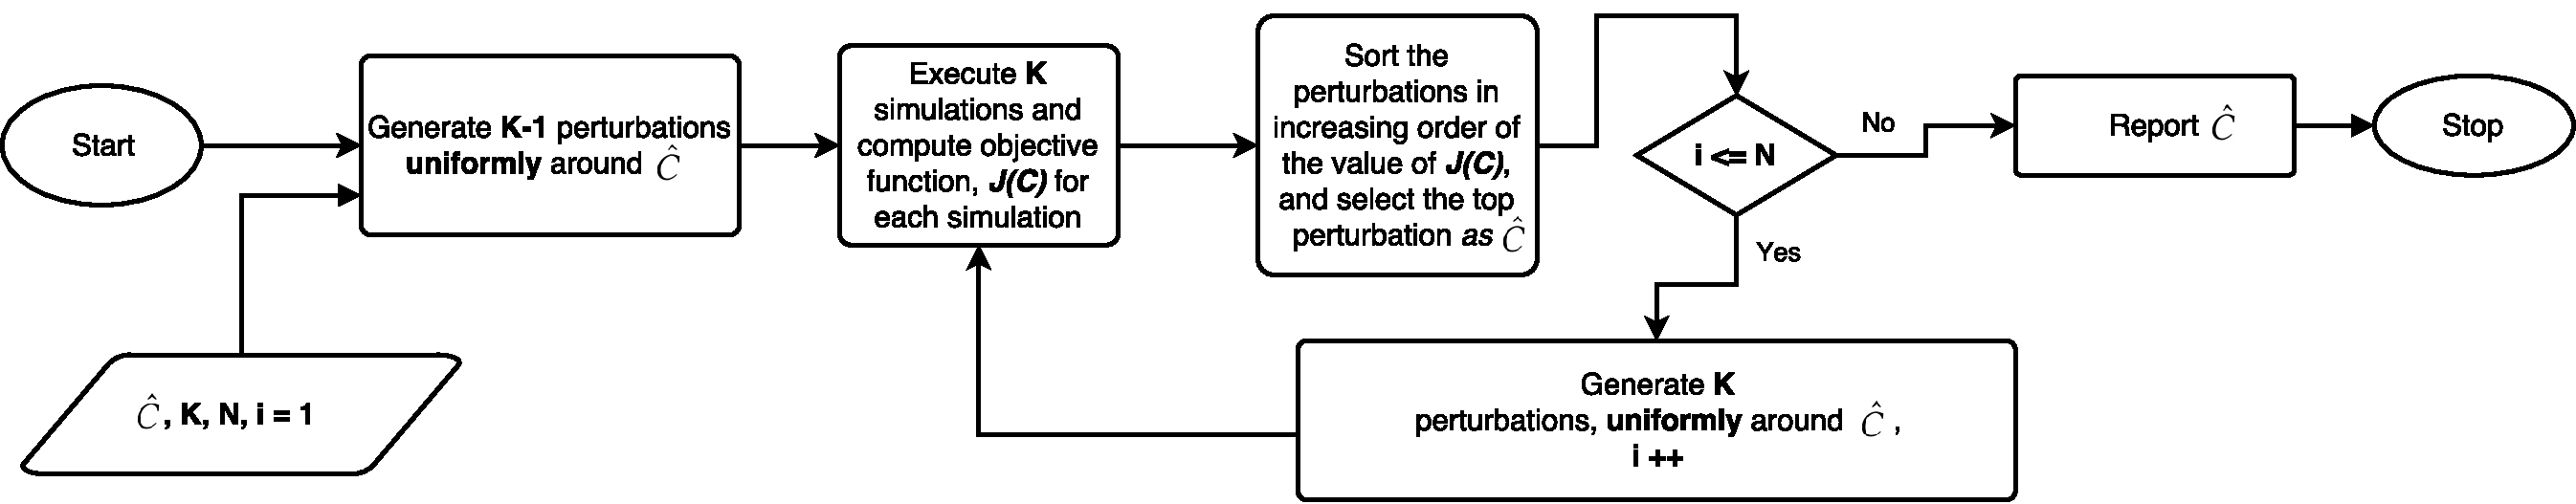
\includegraphics[width=\textwidth]{figures/ngd.pdf}
    \caption{Flow chart of numerical gradient descent for behavior model calibration}
    \label{fig:ngd}
    \end{figure}
    \begin{figure}[H]
    \centering
    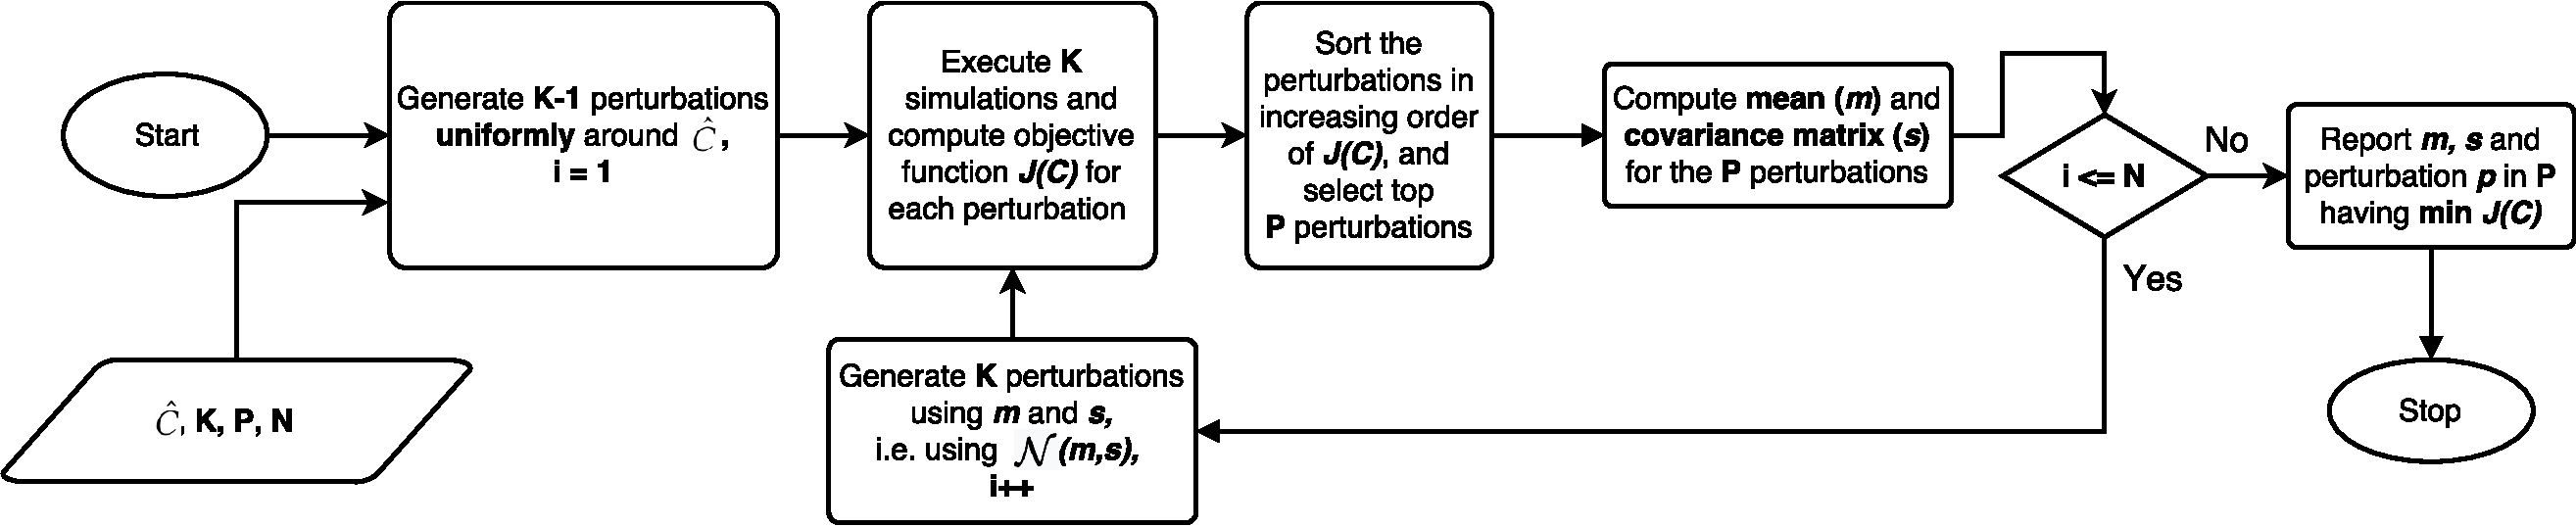
\includegraphics[width=\textwidth]{figures/cem.pdf}
    \caption{Flow chart of CE method for behavior model calibration}
    \label{fig:cem}
    \end{figure}
    \subsection{Numerical gradient descent for behavior model calibration} 
    In this approach, we begin with a random cost vector $\hat{C}$ and generate $K-1$ cost perturbations uniformly around $\hat{C}$. This can be achieved by sampling $K-1$ points uniformly from the surface of an $n-sphere$ centered at $\hat{C}$, where $n = 351$ is the dimensionality of $\hat{C}$. The $K$ cost vectors (i.e. $\hat{C}$ along with $K-1$ perturbations) form the set of candidate optimal cost vectors which are used to parametrize the agent decision making model in $K$ Episimdemics influenza simulations. In each of the $K$ simulations, agents employ the corresponding cost vector along with the ODE SEIR model to decide on behaviors as influenza and information propagate through the social contact network. Each of the $K$ simulations result in a distribution of behaviors. Thus, we can compute the objective function defined in equation (\ref{eqn:objfn}) for each of the $K$ cost vectors and compute the optimal cost vector $C^*$ out of the $K$ cost vectors which has the minimum value of $J(C)$. We then generate $K-1$ new cost vectors around $C^*$ and repeat this process over $N$ iterations to get successively better optimal cost vectors, or until the value of the objective function $J(C)$ falls below a particular threshold. Figure~\ref{fig:ngd} shows the flow chart of the NGD algorithm applied to behavior model calibration.
    
    \subsection{Cross entropy method for behavior model calibration}
    An issue with NGD is that of slow convergence. One way to achieve faster convergence is to use a fast Monte Carlo-based combinatorial optimization algorithm like the Cross Entropy (CE) method~\cite{kroese2013cross,stulp2012path}. The CE method operates by generating a random data sample using a particular mechanism (e.g., sampling from a Gaussian distribution), followed by updating the parameters of the mechanism (e.g., updating the mean and variance of the Gaussian distribution) to produce a ``better'' sample in the next iteration. In the case of using CE method for behavior model calibration, once again we begin with a random cost vector $\hat{C}$ and generate $K-1$ perturbations uniformly around $\hat{C}$ from the surface of an $n-sphere$ centered at $\hat{C}$. The $K$ perturbations are used to parametrize the agent decision-making model in $K$ Episimdemics influenza simulations. Similar to NGD, we then compute the value of objective function $J(C)$ for each of the K perturbations. However, instead of selecting one perturbation with the minimum value of $J(C)$, we select $P$ perturbations that have the least values for the objective function $J(C)$ out of the $K$ perturbations. Next, we compute the mean $m$ and covariance matrix $S$ for these top $P$ perturbations and use the multi-variate Gaussian distribution $\mathcal{N}(m,S)$ to once again generate $K$ perturbations for use in the next iteration. We continue this process for $N$ iterations before reporting the results. Figure~\ref{fig:cem} shows the flow chart for the CE method applied to behavior model calibration.
    
    \subsection{Smoothed cross entropy method for behavior model calibration}
    In our experiments we observed that the covariance matrix $S$ computed by the CE method quickly converged to zeros at an early stage of the optimization. This is analogous to the algorithm being stuck in a local minimum. In order to prevent this behavior of the CE method, we use a smoothing parameter $\alpha$ to update the mean $m_t$ and covariance matrix $S_t$ on the $t^{th}$ iteration~\cite{mannor2003cross}.
    \begin{align}
        m_t &= \alpha  \hat{m} + (1-\alpha)  m_{t-1}
    		\label{eqn:smean}
    \end{align}
    \begin{align}
    		S_t &= \alpha  \hat{S} + (1-\alpha)  S_{t-1}
    		\label{eqn:scovmat}
    \end{align}
    
    Here, $\hat{m}$ is the mean and $\hat{S}$ the covariance matrix of the top $P$ perturbations computed for iteration $t$, $m_{t-1}$, $S_{t-1}$ is the mean and covariance matrix computed for the last iteration (i.e. $t-1$) and $\alpha$ is the smoothing parameter such that $0 < \alpha < 1$. 
    
    \subsection{Using quantal best response for agent decisions}
    Upon closer analysis of our calibration results from the optimization approaches discussed until now, we found that we were able to match the distribution of the $14$ behavioral actions observed in the survey with those observed in the simulation to a great extent. Although the distribution of the $351$ behaviors did not seem to match very well between the survey and the epidemic simulation. To address this problem we, modified a few aspects of the Smoothed-CE method, which resulted in much better calibration of the behavior distributions.
    
    First, we replaced the mean squared error (MSE) objective function with a sum of squared error (SSE) objective function. This modification was aimed at making the loss more sensitive to large differences between the behavior proportions observed in the simulation and the outbreak survey. Since, the MSE essentially averages all the squared errors; it starts to reduce as soon as some of the errors drop to zero. The reduction in MSE is also affected by the number of behaviors. In other words as the number of behaviors grow, the MSE value reduces substantially because of the $2 * |C|$ term in the denominator. On the other hand, as the SSE does not average the squared error values, it is more sensitive to large errors and less sensitive to the number of behaviors. The new objective function is as follows,
    \begin{align}
        J(C) &= \sum_{b \in B}\bigg[ N_{C_b} - N_{b} \bigg]^2
    	\label{eqn:objfn3}
    \end{align}
    
    Second, past work in the cognitive sciences and behavioral game theory suggests that instead of selecting the behavior with the maximum value (or utility), agents respond stochastically to their incentives. This means that agents select high value behaviors with high probability and low value behaviors with low probability~\cite{wright2014level}. This model of behavioral response is called the Quantal Best Response (QBR), and given a value function $V_d$ to quantify the utility associated with a behavior $b$ on a day $d$, an agent`s behavior choice is determined by the strategy $\mathbb{S}$, which can be defined as follows,
    \begin{align}
        \mathbb{S}(b) &= \frac{\exp (\lambda * V_d(b)) }{ \sum\limits_{b' \in B} \big[ \exp(\lambda * V_d(b')) \big]}
    	\label{eqn:qbr}
    \end{align}
    Here, $\lambda$ refers to the precision or the agent`s sensitivity to differences in the values associated with different behaviors. When $\lambda = 0$, the strategy $\mathbb{S}$ would always be equal to $1$, resulting in the agent`s behavior choice to be uniformly distributed over all possible behaviors in $B$. Conversely, as $\lambda \rightarrow \infty$, the strategy $\mathbb{S}$ converges to the best behavior, instead of being a distribution over all the behaviors. This leads to the agent`s behavior choice always being the behavior $b$, that maximizes $V_d(b)$, similar to our earlier approach (i.e., equation~\ref{eqn:optb}). In this work, we use $\lambda = 1$, so as to allow an agent`s behavior choice to be stochastic, while being aligned with the quantal best response principle. This means that behaviors having a high value would be selected with a higher probability and behaviors with a low value would be selected with a low probability.
    
    Therefore, the QBR method gives us a probability distribution over the behavior space, from which we can sample a single behavior using Inverse Transform Sampling~\cite{wiki:its} and assign the sampled behavior to the decision making agent. The agent in the epidemic simulation then adopts the assigned behavior. Note that the rest of the optimization process remains unchanged, and we only apply the QBR method alongside the Smoothed-CE optimization method in this work. 
    
    \section{Epidemic Calibration}
    The last step for solving the \textsc{BehavAssign} problem is to calibrate the simulated epidemic outcome with that observed in the real world. Although there can be multiple epidemic outcomes, all of which can be calibrated, in this work we only calibrate the proportion of real world population which got infected by the flu in the real-world $I$, with the proportion of agents which get infected in the epidemic simulation $\hat{I}$. We do this by adjusting the value of the transmission rate $\rho$ parameter of the inter-host disease propagation model (discussed in section~\ref{sec:4.2}). We considered the target proportion $I$ to be $0.33$ or $33\%$ of the total population and adjusted $\rho$, such that $\hat{I} \approx 0.33$. The value of $\rho$ which resulted in $\hat{I} \approx 0.33$ came out to be $5.528 \times 10^{-5}$. After implementing and calibrating the behavior model, the $\hat{I}$ in the simulation reduced from $0.33$ to $0.006$. This was due to the agents deciding and adopting preventive behaviors against Influenza in the simulation. In order to calibrate the simulated epidemic and complete the last step of the \textsc{BehavAssign} problem, we increased $\rho$, until the simulation once again started producing $\hat{I} \approx 0.33$. This value of $\rho$ was $1.1332 \times 10^{-4}$ and this is the $\hat{\rho}$ we wanted to find as one of the objectives of the \textsc{BehavAssign} problem. The  Figure~\ref{fig:epicalib} shows the cumulative infections seen in the simulation before and after the epidemic calibration step with the behavior model in-place. Note that the value $\hat{I}$ corresponds to the proportion of infections at the end of the simulation duration. With epidemic calibration, we see that this value becomes close to the target of $0.33$, on the other hand, without calibration the epidemic dies out early in the simulation, leading to the almost flat cumulative infections curve. 
    
    \begin{figure}
    \centering
    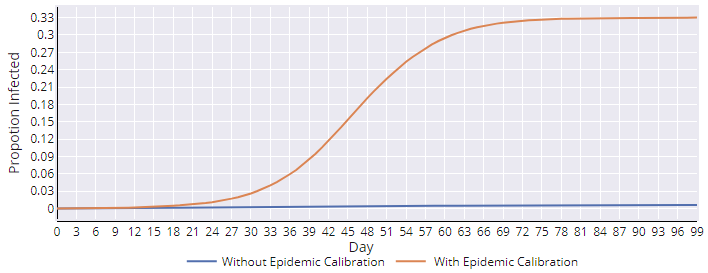
\includegraphics[width=\textwidth]{figures/epicalib.png}
    \caption{Cumulative infections produced by the simulation with and without epidemic calibration step.}
    \label{fig:epicalib}
    \vspace{-0.1in}
    \end{figure}
    
    If we do not consider human behavior when simulating epidemics, the epidemic parameters, (e.g., $\rho$) compensate for the effect of human behavior on the real-world epidemic. This might be sufficient if we are only interested in assessing the impact of non-behavioral interventions on the epidemic. However, given that most of the interventions in the real world are behavioral interventions, involving active decision making by individuals, having a behavior model in a simulation can allow us to evaluate behavioral interventions and their impact on infectious disease epidemics. 
    
    \section{Reasonability of generated behavior}
    Another important aspect when it comes to assigning human behavior to agents in a simulation is that of reasonability. While people may make sudden changes in their behavior upon certain events, for example a natural disaster or an emergency notification, past literature~\cite{ariely2008predictably} suggests that people in general stick with their behaviors. We can think of this as an example of a reasonability constraint on the behavior assigned to an agent. The agent decision-making model allows us to inspect and enforce such constraints on its behavior assignment results. For example, we can enforce a constraint that only allows an agent to switch from its current behavior $b_i$ to alternate behavior $b_j$, if the two behaviors differ by $l$ constituent actions or less, i.e. $|b_i - b_j| \le l$. 
    
    In our last calibration experiment, with the notion of quantal best response (QBR), we also apply a simple constraint on the behavior generated by the behavior model. The constraint that once an agent has decided on a behavior $b$, they stick with it. This constraint is well aligned with past literature in behavioral economics~\cite{ariely2008predictably}. We can also incorporate more complex reasonability constraints in the \textsc{BehavAssign} problem itself. For instance, we can modify the objective function defined in~\ref{obj-func} as follows:
    \begin{align*}
        \min \upalpha \bigg(\sum_{i=1}^{m}|p_i - \hat{p_i}|\bigg) + \upbeta \bigg(|I - \hat{I}| \bigg) + \upgamma \bigg(\frac{1}{n} \sum_{j=1}^{n} t_j \bigg) \\
        \sum_{i=1}^{m} \hat{p_i} = 1.0 \\
        \hat{\rho} \ge 0.0\\
        \upalpha, \upbeta, \upgamma \in [0, 1]
    \end{align*}
    Here, $t_j$ is the number of times the behavior of agent $a_j$ changed in the simulation and the third term of the objective function would help minimize the mean number of transitions in an agent`s behavior in the simulation. This formulation allows us to incorporate such complex reasonability constraints into the behavior calibration process. However, we do not explore these reasonability constraints in the current work. In the next chapter, we present the behavior calibration results obtained using the four behavior model calibration methods we have discussed in this chapter. 
    
	\chapter{Results} \label{ch:results}
	\begin{figure}
    \centering
    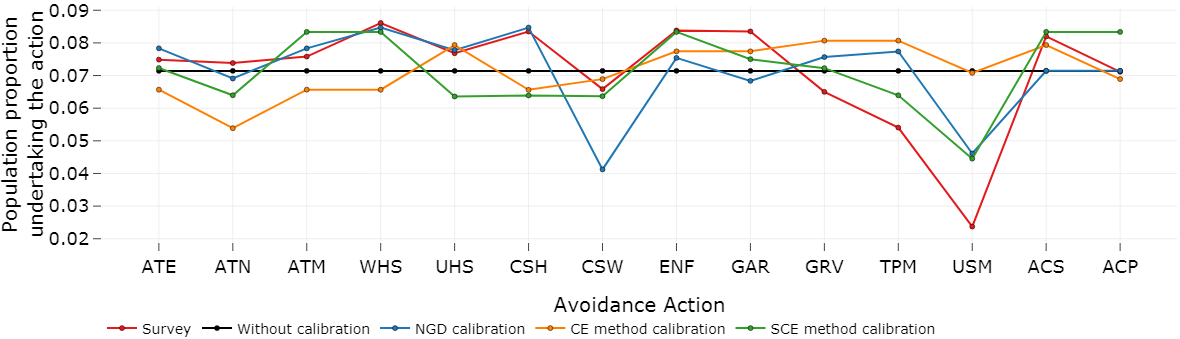
\includegraphics[width=\textwidth]{figures/marginals.png}
    \caption{Distribution of influenza avoidance action choices observed in the survey, those generated by an uncalibrated agent decision model and those generated by the three calibration approaches}
    \label{fig:marginals}
    \end{figure}
    
    \begin{figure}
    \centering
    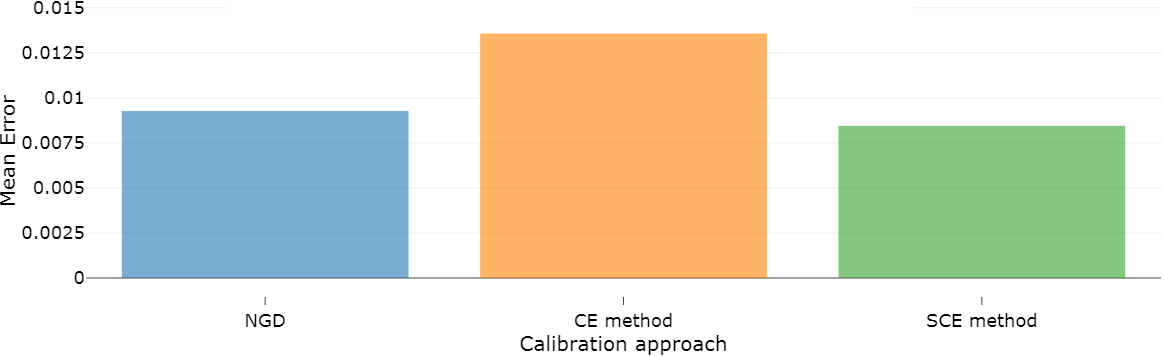
\includegraphics[width=\textwidth]{figures/meanerrors.png}
    \caption{Mean error between the avoidance action distribution observed in the survey and those generated by the three calibration approaches}
    \label{fig:mean-errors}
    \vspace{-0.1in}
    \end{figure}
    
    In order to compare the calibration results obtained using the different calibration approaches, we initialized each of them with a common $\hat{C}$ vector, with each element in $\hat{C}$ being equal to a constant $c$ (we kept $c=0.5$ in our experiments). We initialized the NGD algorithm with $K=15$ and executed it for $N=2000$ iterations, which resulted in a $J(C)$ value of $1.651 \times 10^{-4}$. The calibration resulted in a mean error of $9.268 \times 10^{-3}$ for the action choice distribution as shown in Figure~\ref{fig:mean-errors}. In order to obtain faster optimization, we experimented with the CE method, initializing it with $K=30$, $P=15$ and executed it for $N=100$ iterations. This resulted in a $J(C)$ value of $2.038 \times 10^{-4}$ and a mean error of $1.3574 \times 10^{-2}$ for the action choice distributions. Although the final objective function value and the mean error obtained using CE method were worse than those obtained using NGD, the CE method substantially reduced the number of iterations (from $2000$ to $100$), which amounts to a $20$ times speedup, since each iteration takes the same amount of time in both the cases. 
    
    We found that the covariance matrix $S$ computed in the CE method converged to zeros on the $30^{th}$ iteration, which stopped the optimization process at an early stage. To address the problem we experimented with the Smoothed-CE (SCE) method, initialized with a smoothing factor $\alpha = 0.5$ and executed it for $N=100$ iterations. This time the calibration process resulted in a $J(C)$ value of $1.6363 \times 10^{-4}$ and a mean error of $8.447 \times 10^{-3}$, which are an improvement over the CE method results and are much closer to the results obtained using NGD. Figure~\ref{fig:marginals} compares the distribution of the action choices observed in the survey responses with those generated by an uncalibrated agent decision model and those generated after calibration using NGD, CE method and SCE method.
    
    \begin{figure}
    \centering
    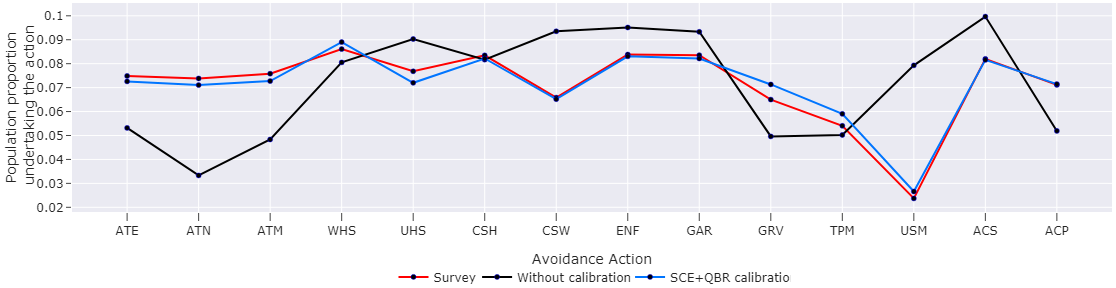
\includegraphics[width=\textwidth]{figures/qbr-marginals.png}
    \caption{Distribution of influenza avoidance action choices observed in the survey, those generated by an uncalibrated agent decision model and those generated by the SCE calibration approach with SSE and QBR modifications.}
    \label{fig:qbr-marginals}
    \end{figure}
    \begin{figure}
    \centering
    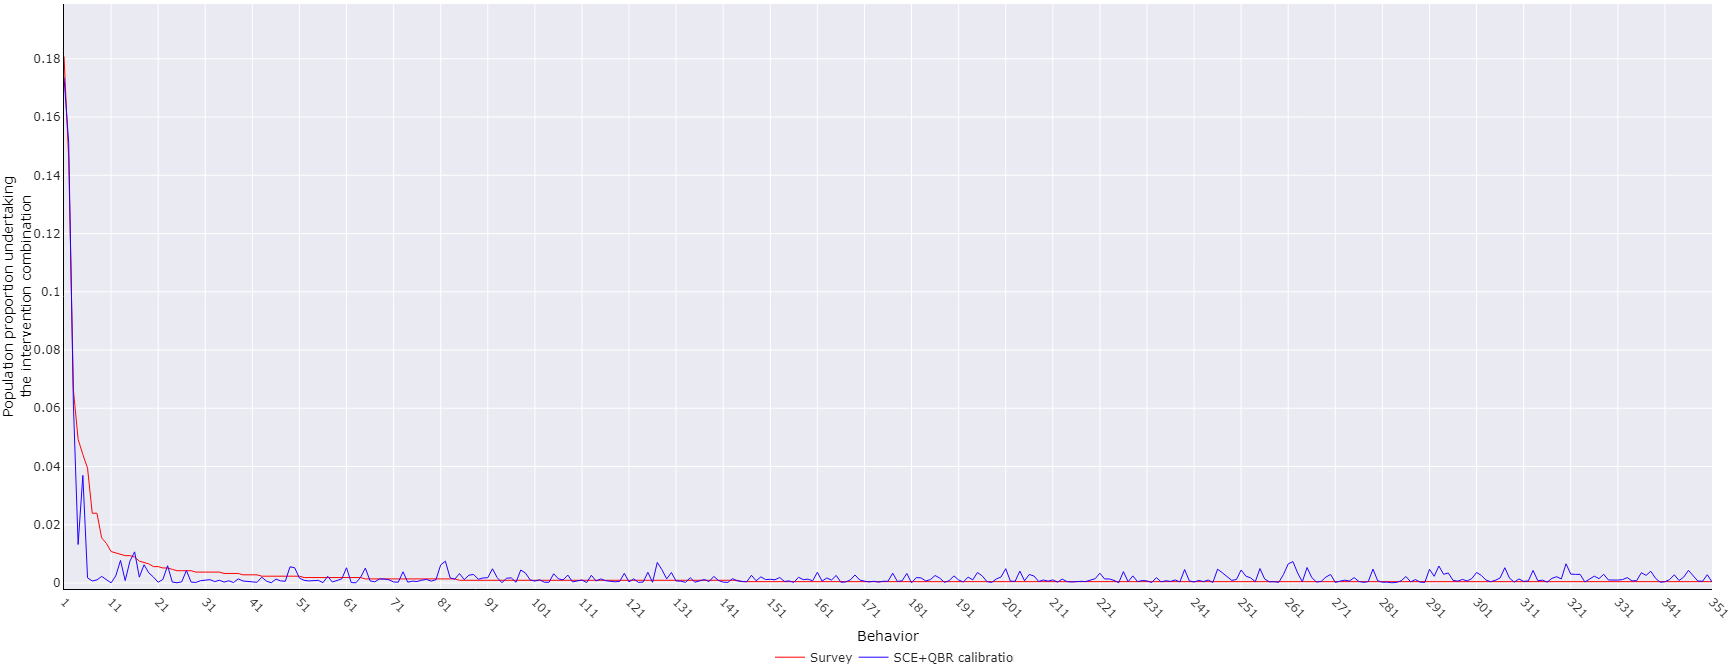
\includegraphics[width=\textwidth]{figures/qbr-joints.png}
    \caption{Distribution of behaviors observed in the survey and those generated by a agent decision model calibrated using SCE calibration approach with SSE and QBR modifications.}
    \label{fig:qbr-joints}
    \end{figure}
    
    Lastly, we executed the Smoothed-CE method with the SSE loss and QBR modifications, and a smoothing factor $\alpha = 0.5$ for $N=43$ iterations which resulted in a SSE of $5.77607 \times 10^{-3}$. The action and behavior calibration results obtained in this experiment are shown in figures~\ref{fig:qbr-marginals} and \ref{fig:qbr-joints}. Out of all the calibration approaches discussed so far, the modified-SCE method resulted in the best calibration in both action and behavior spaces.
    
    \chapter{Conclusions and Future Work} \label{ch:conclusions}
	In this work, we have shown how to use survey data to calibrate an agent decision-making model for a large-scale flu epidemic simulation. The technique is not specific to infectious diseases, so it applies to surveys and simulations in general, though it requires a domain-specific decision-making model for each agent akin to the SEIR model used here. The objective of this work was to simulate populations of behaving agents, which match the behaving individuals in real populations and exhaustive parameter sweeps for the optimization techniques used in the calibration might improve the results reported here. Additionally, other gradient free optimization techniques like Nelder-Mead Simplex or CMA-ES might lead to different amounts of calibration and performance. In this work, we compared three optimization techniques, although experimentation with other techniques may lead to better or worse results. However, all of these aspects are independent of the basic behavior model calibration approach discussed in this work. 
	
	While we could construct regression models to predict the probability of an agent adopting a particular behavior using the survey, this does not give us a model of agent decision-making. Our approach develops a model of agent decision-making, which can be interpreted, inspected and compared with other models in the literature. We have developed a very general and practical representation of behaviors for simulations. The behaviors, like options~\cite{sutton99options}, are higher level descriptions that have initiation and termination conditions, and a policy which can alter the actions (in the form of the activity schedule) and the states (in the form of the FSMs) of each agent. This general representation can be adapted to most social simulation scenarios. Of course, there are scenarios where FSMs will not be powerful enough to represent the agent's state, but in that case, the behavior model will just have to specify how to work with the more complex representation of state. 
	
    There are many opportunities for extending this work. In general, the scientific process of gathering data through a survey and then developing a model with it proceeds in an abductive loop in the sense of Peirce~\cite{peirce57abduction}. Thus one of the most useful purposes of such simulations is in the ``context of discovery'', i.e., to generate new hypotheses. By integrating behavior models, we can now generate detailed forecasts of behavior adoption, which can then be confirmed (or disconfirmed) through new surveys. The goal is to bring rapidity and rigor into the study of human behavior in context. This need to be done by making the behavior modeling process as data driven as possible and then using the models to drive further hypothesis generation and data collection. 
    
    There are several limitations to our study. First, human behavior, disease dynamics, and policy decisions co-evolve and in this study, we have only calibrated the behavior followed by one aspect of the disease, i.e., the total number of infections. We can alternatively look at the \textsc{BehavAssign} problem as a multicriteria optimization where we simultaneously optimize behavior model and disease model parameters. In this case, we might obtain multiple Pareto optimal solutions, which can then be analyzed and validated against real-world observations. Second, in this thesis we have assumed that the behavioral distribution observed for the entire U.S. will match the behavior distribution observed in a much smaller and less diverse geographic area of Montgomery County, VA. This was primarily because we did not have enough data points in the survey for Montgomery, VA, we only had 63 survey records for the state of Virginia. However, we can use the same approach given that we have enough data available for the geographic area we are trying to simulate. Third, there can be many other phenomenon that can impact an individual`s decisions about preventive actions against a disease. Each of these factors can have different modes of diffusion among the population and each individual can respond differently to each of these phenomena. For example, it might be desirable to model aspects such as word of mouth, disease awareness advertising and emotion or fear contagions~\cite{epstein08coupled}. Additionally, we can model the information contagion process in a more careful and data-driven way. Fourth, we can analyze individual agent trajectories as well as behavior forecasts done by the calibrated behavior model against observations in the real world. Although it might be difficult to validate individual trajectories against those observed in the real-world because of the shear difficulty in collecting people`s behavioral trajectories during epidemics, the aggregate-level behavioral distributions may be validated against distributions observed in a subsequent outbreak survey. Finally, there may not be a static model of human behavior that can be inferred once and used thereafter. The feedback between human behavior, disease dynamics, and policy decisions co-evolving in the system also needs to be accounted for. This will require modeling how behaviors change over time and under different circumstances. 
    
	% This is the standard bibtex file. Do not include the .bib extension in <bib_file_name>.
	% Uncomment the following lines to include your bibliography 
	%\bibliography{<bib_file_name>}
	%\bibliographystyle{plainnat}   

% 	% This formats the chapter name to appendix to properly define the headers
% 	\appendix

% 	% Add your appendices here.  You must leave the appendices enclosed in the appendices 
% 	% environment in order for the table of contents to be correct.
% 	\begin{appendices}
% 		\chapter{First Appendix} \label{app:appendix_one}
% 			\section{Section one} \label{ase:app_one_sect_1}
% 				\lipsum[1-3]
% 			\section{Section two} \label{ase:app_one_sect_2}
% 				\lipsum[1-3]
% 		\chapter{Second Appendix} \label{app:appendix_two}
% 			\lipsum[2]
% 	\end{appendices}
\bibliographystyle{ACM-Reference-Format}
\bibliography{references}
\end{document}


%****************************************************************************
% Below are some general suggestions for writing you dissertation
%
% 1. Label everything with a meaningful prefix so that you
%    can refer back to sections, tables, figures, equations, etc.
%    Usage \label{<prefix>:<label_name>} where some suggested
%    prefixes are:
%			ch   : Chapter
%     se   : Section
%     ss   : Subsection
%     sss  : Sub-subsection
%			app  : Appendix
%     ase  : Appendix section
%     tab  : Tables
%     fig  : Figures
%     sfig : Sub-figures
%     eq   : Equations
%
% 2. The VTthesis class provides for natbib citations.  You should 
%    in one or more *.bib bibtex files and save them in your working 
%    directory. Suppose you have two bib files: some_refs.bib and 
%    other_refs.bib.  Then your bibliography line to include them
%    will be:
%      \bibliography{some_refs,other_refs}
%    where multiple files are separated by commas.  In the body of 
%    your work you can cite your references using natbib citations.
%    Examples:
%      Citation                     Output
%      -------------------------------------------------------
%      \cite{doe_title_2016}        [18]
%      \citet{doe_title_2016}       Doe et al. [18]
%      \citet*{doe_title_2016}      Doe, Jones, and Smith [18]
%
%    For a complete list of options see
%      https://www.ctan.org/pkg/natbib?lang=en
%
% 3. Here is a sample table.  Notice that caption is centered at the top. Also
%    notice that we use booktabs formatting.  You should not use vertical lines
%    in your tables.
% 
%				\begin{table}[htb]
%					\centering
%					\caption{Approximate computation times in hh:mm:ss for full order versus reduced order models.}
%					\begin{tabular}{ccc}
%						\toprule
%						& \multicolumn{2}{c}{Computation Time}\\
%						\cmidrule(r){2-3}
%						$\overline{U}_{in}$ m/s & Full Model & ROM \\
%						\midrule
%						0.90 & 2:00:00 & 2:08:00\\
%						0.88 & 2:00:00 & 0:00:03\\
%						0.92 & 2:00:00 & 0:00:03\\
%						\midrule
%						Total & 6:00:00 & 2:08:06\\
%						\bottomrule
%					\end{tabular}
%					\label{tab:time_rom}
%				\end{table}
% 
% 4. Below are some sample figures.  Notice the caption is centered below the
%    figure.
%    a. Single centered figure:
%					\begin{figure}[htb]
%						\centering
%						\includegraphics[scale=0.5]{my_figure.eps}
%						\caption{Average outlet velocity magnitude given an average input velocity magnitude of 0.88 m/s.} 
%						\label{fig:output_rom}
%					\end{figure}
%    b. Two by two grid of figures with subcaptions
%					\begin{figure}[htb]
%						\centering
%						\begin{subfigure}[h]{0.45\textwidth}
%							\centering
%							\includegraphics[scale=0.4]{figure_1_1.eps}
%							\caption{Subcpation number one}
%							\label{sfig:first_subfig}
%						\end{subfigure}
%						\begin{subfigure}[h]{0.45\textwidth}
%							\centering
%							\includegraphics[scale=0.4]{figure_1_2.png}
%							\caption{Subcpation number two}
%							\label{sfig:second_subfig}
%						\end{subfigure}
%
%						\begin{subfigure}[h]{0.45\textwidth}
%							\centering
%							\includegraphics[scale=0.4]{figure_2_1.pdf}
%							\caption{Subcpation number three}
%							\label{sfig:third_subfig}
%						\end{subfigure}
%						\begin{subfigure}[h]{0.45\textwidth}
%							\centering
%							\includegraphics[scale=0.4]{figure_2_2.eps}
%							\caption{Subcpation number four}
%							\label{sfig:fourth_subfig}
%						\end{subfigure}
%						\caption{Here is my main caption describing the relationship between the 4 subimages}
%						\label{fig:main_figure}
%					\end{figure}
%
% 5. You should place your images and figures in a subdirectory.  You can 
%    then tell Latex to look for all your images there using:
%      \graphicspath{{figures/}}
%    Note: you must have both sets of curly braces and include the final
%          directory /
% 
%----------------------------------------------------------------------------
%
% The following is a list of definitions and packages provided by VTthesis:
%
% A. The following packages are provided by the VTthesis class:
%      amsmath, amsthm, amssymb, enumerate, natbib, hyperref, graphicx, 
%      tikz (with shapes and arrows libraries), caption, subcaption.
%      listings, verbatim
%
% B. The following theorem environments are defined by VTthesis:
%      theorem, proposition, lemma, corollary, cojecture
% 
% C. The following definition environments are defined by VTthesis
%      definition, example, remark, algorithm
%
%----------------------------------------------------------------------------
%
%  I hope this template file and the VTthesis class will keep you from having 
%  to worry about the formatting and allow to focus on the actual writing.
%  Good luck and happy writing.
%    Alan Lattimer, VT, 2016
%
%****************************************************************************





